%\documentclass{report}
\documentclass[nobib]{tufte-book}

\usepackage{standalone}

\usepackage{calc}

%\usepackage[bookmarks=true]{hyperref}

% symbols
\usepackage{amsmath} % assumes amsmath package installed
\usepackage{amssymb} % for \square
% non-italicized math subscripts
\newcommand{\ms}[1]{\mbox{\scriptsize #1}}

% from http://tex.stackexchange.com/a/5255
\DeclareMathOperator*{\argmin}{arg\,min}

% algorithm stuff
\usepackage{algorithm}
\usepackage[noend]{algpseudocode}

\usepackage{array}
\usepackage{graphicx}
%\usepackage{subcaption}
\usepackage[caption=false]{subfig} %[caption=false]
\usepackage{float} % for side-by-side figures?
% http://tex.stackexchange.com/a/95357

\usepackage{setspace}

\floatstyle{plain}
\newfloat{genericfloat}{t}{gflt}

\usepackage{tikz}
\usetikzlibrary{arrows,backgrounds,calc,patterns,positioning,shapes,decorations.pathmorphing}

% plots
\usepackage{pgfplots}

% pretty tables
\usepackage{multirow}
\usepackage{booktabs}

% custom title page
\usepackage{titling}

% for adjustwidth
\usepackage{changepage}

% include \paragraph as numbered
\setcounter{secnumdepth}{3}
\setcounter{tocdepth}{1} % 3

%\def\hidenotes{}
% list of commenters
\newcommand{\ssnote}[1]{{\xxnote{SS}{red}{#1}}}
\newcommand{\cdnote}[1]{{\xxnote{CD}{blue}{#1}}}
\newcommand{\mknote}[1]{{\xxnote{MK}{green}{#1}}}
% implement conditional notes (turn on/off with \hidenotes above)
\newcommand{\xxnote}[3]{}
\ifx\hidenotes\undefined
  \usepackage{color}
  \renewcommand{\xxnote}[3]{\color{#2}{#1: #3}}
\fi

% wide page for side by side figures, tables, etc
% see http://tex.stackexchange.com/a/154766
\newlength{\offsetpage}
\setlength{\offsetpage}{1.5in}
\newenvironment{widepage}
   {\begin{adjustwidth}{-\offsetpage}{-\offsetpage}%
    \addtolength{\textwidth}{2\offsetpage}}%
{\end{adjustwidth}}

% theorems
\newtheorem{invariant}{Invariant}
\newtheorem{theorem}{Theorem}
\newtheorem{proposition}{Proposition}
\newtheorem{lemma}{Lemma}
% from http://www.maths.tcd.ie/~dwilkins/LaTeXPrimer/Theorems.html
\newenvironment{proof}[1][Proof]{\begin{trivlist}
   \item[\hskip \labelsep {\bfseries #1}]}{\hfill$\square$\end{trivlist}}

\title{Efficient Manipulation Task Planning via\\
   Reuse-Informed Optimization of Planning Effort}
\author{Christopher M. Dellin}
\date{\today}

\renewcommand{\maketitlehooka}{
\begin{fullwidth}
}

\renewcommand{\maketitlehookd}{
\begin{center}
\vspace{0.7in}
The Robotics Institute\\
Carnegie Mellon University\\
Pittsburgh, PA 15213\\
\vspace{0.7in}
\textbf{Thesis Committee:}\\
Siddhartha Srinivasa, CMU RI (Chair)\\
Anthony Stentz, CMU RI\\
Maxim Likhachev, CMU RI\\
Lydia Kavraki, Rice University\\
%\vspace{0.7in}
%\emph{Submitted in partial fulfillment of the requirements\\
%for the degree of Doctor of Philosophy.}
\end{center}
\end{fullwidth}
}

\begin{document}

\maketitle

%\begin{abstract}
\begin{fullwidth}
\begin{adjustwidth}{1in}{1in}

{\LARGE \emph{Abstract}}

\vspace{0.2in}

In order to assist humans
with dangerous or menial tasks,
autonomous robots will need to
act under significant time and energy constraints.
At task time,
the amount of effort a robot spends planning directly
detracts from its total performance.
Manipulation tasks, however, present challenges
to efficient motion planning.
They are often tightly coupled --
while moving an object can be decomposed into
steps (reach, grasp, transfer, release),
each step requires choices (e.g. which grasp),
and committing to a bad choice
can render subsequent steps difficult;
this encourages longer planning horizons.
However,
an articulated robot
situated within a geometrically complex and dynamic environment
induces a high-dimensional configuration space
in which it is expensive to test for valid paths.
And since multi-step plans
require paths in changing valid subsets of configuration space,
it is difficult to reuse computation across steps
or maintain caches between tasks.

We focus on a motion planning approach for coupled multi-step
manipulation problems that is efficient over the entire task
(including both planning and execution).
We contend that the problem's cost structure
favors explicit handling of
both graph representation and task effort optimization,
and propose a graph search algorithm which captures these insights
given a model of planning effort.
We offer methods for roadmap construction
which seek to balance completeness with efficiency at task time.
We then unify previous work examining configuration space structure of
related problems (e.g. multi-step manipulation)
into a general set-theoretic formulation
which suggests a planning effort model
to be exploited by our roadmap search algorithm,
yielding a motion planner which
efficiently reuses computation between queries.
We also present a task planner
that maps a task decomposition into queries to our motion planner.
Our insights yield complementary components
which, taken together,
consitute an efficient approach to planning manipulation tasks.

This thesis proposes a heavy emphasis on experimental evaluation
of the individual constituent algorithms
and the approach as a whole.
We will compare against
state-of-the-art task and motion planners
on multiple robotic platforms,
in applications from home table clearing
to remote disaster response.
We also provide open-source implementations of our algorithms.

\end{adjustwidth}
\end{fullwidth}
%\end{abstract}

\tableofcontents

\chapter{Introduction}

The steady advancement of technology
has automated an increasing variety of menial or dangerous tasks
previously performed by humans.
Computer algorithms now trade our stocks,
route our telephone calls and packages,
and fly our planes,
and simple machines clean our clothes and wash our dishes.

More complex tasks require complex robots with many
degrees of freedom.
Manipulation tasks, in particular,
present challenges in many areas including
perception, symbolic reasoning, and motion planning.
Successful applications have so far been largely
confined to large-scale manufacturing domains,
whose prescribed and structured environments
allow these challenges to be overcome.

However,
manipulation tasks such as clearing a kitchen table
or moving debris in a dangerous disaster scenario
can not yet be planned for quickly and reliably.
\begin{quote}
\emph{%
This thesis proposes an
efficient and robust motion planning approach
well-suited
to articulated robots
performing recurring manipulation tasks
in dynamic, unstructured environments.
}
\end{quote}

We outline the general structure of manipulation tasks
in Chapter~\ref{chap:formulation}.
There are three principal challenges inherent in
human-scale manipulation tasks
that must be addressed by planning approaches,
which we review here.

\textbf{Challenge 1: Manipulation Tasks must be Resource-Efficient}

Autonomous systems performing manipulation tasks are
resource-constrained.
If a home robot takes thirty minutes to clear a table,
or a disaster response robot exhausts its battery ten minutes
into its mission,
these robots will not see widespread use.
These metrics are only meaningful
when applied across the entire task,
from assignment to completion.

In order to accomplish such a manipulation task,
an autonomous robot must expend two types of effort.
First, it must allocate computation to \emph{plan}
a sequence of motions that will acheive the task.
Planning costs are dominated by \emph{validity checking} --
e.g. checking whether configurations are free from collision.
Second, it must \emph{execute} these motions using its actuators.
Typically, there is a tradeoff between these two;
spending more effort during planning produces paths that are
cheaper to execute.

Robots performing real-world human-scale manipulation tasks
tend to expend comparable effort in these two areas
(see Figure~\ref{fig:plan-exec-cost}).
While some approaches (e.g. anytime planning) partially capture
this tradeoff,
our approach explicitly optimizes for both planning
and execution effort
-- what we call the task's \emph{ensemble effort}.
We apply this reasoning to explicit graphs
with the E$^8$ search algorithm (Chapter~\ref{chap:inflate})
which determines an effort allocation between planning and execution
in order to minimize total task cost.

In order to solve planning problems in continous configuration spaces,
we borrow heavily from roadmap techniques for graph construction.
The application of our ensemble effort algorithm to such roadmaps,
the E$^8$-PRM (Chapter~\ref{chap:graphs-in-continuous}),
maintains efficiency through an
incremental densification approach
motivated by approximating the probabalistic spatial correlation of
$\mathcal{C}_{\mbox{\scriptsize free}}$.

{
\setlength{\offsetpage}{0.5in}
\begin{figure}[t]
\begin{widepage}
\begin{center}
   \begin{subfigure}[b]{1.4in}
      \begin{center}
      \includegraphics{build/intro-cost-herb}
      \end{center}
      \caption{\textsc{Herb} Home Robot}
   \end{subfigure}%
   \quad%
   \begin{subfigure}[b]{2.0in}
      \begin{center}
      \includegraphics{build/intro-cost-chimp}
      \end{center}
      \caption{\textsc{Chimp} Disaster Response Robot}
   \end{subfigure}%
   \quad%
   \begin{subfigure}[b]{2.0in}
      \begin{center}
      \includegraphics{build/intro-cost-axis}
      \end{center}
      \caption{Planning vs. Execution Cost}
   \end{subfigure}
   \caption{For manipulation tasks,
      both the \textsc{Herb} \cite{srinivasa2012herb20}
      and \textsc{Chimp} \cite{stentz2014chimp} robots
      incur comparable cost (e.g. time or energy)
      during planning and execution.
      Our approach considers both explicitly.}
   \label{fig:plan-exec-cost}
\end{center}
\end{widepage}
\end{figure}
}

\textbf{Challenge 2: Incongruent Sub-Problems Impede Reuse.}

{
\setlength{\offsetpage}{0.75in}
\begin{figure}[t]
\begin{widepage}
\begin{center}

\begin{subfigure}[t]{0.19\linewidth}
\centering
\includegraphics[width=\columnwidth]{figs/testherb-a.png}
\caption{Start config}
\end{subfigure}
\begin{subfigure}[t]{0.19\linewidth}
\centering
\includegraphics[width=\columnwidth]{figs/testherb-b.png}
\caption{Part 1 in $X_1$}
\end{subfigure}
\begin{subfigure}[t]{0.19\linewidth}
\centering
\includegraphics[width=\columnwidth]{figs/testherb-c.png}
\caption{Part 2 in $X_2$}
\end{subfigure}
\begin{subfigure}[t]{0.19\linewidth}
\centering
\includegraphics[width=\columnwidth]{figs/testherb-d.png}
\caption{Part 3 in $X_3$}
\end{subfigure}
\begin{subfigure}[t]{0.19\linewidth}
\centering
\includegraphics[width=\columnwidth]{figs/testherb-e.png}
\caption{End config}
\end{subfigure}

\vspace{0.1in}

   \begin{subfigure}[b]{4.0in}
      \begin{center}
      \includegraphics{build/intro-subprob-cspace}
      \end{center}
      \caption{Plan sequences
         within distinct free $\mathcal{C}$-subsets
         from the problem above.}
   \end{subfigure}%
   \quad%
   \begin{subfigure}[b]{2.0in}
      \begin{center}
      \includegraphics{build/intro-subprob-axis}
      \end{center}
      \caption{Single vs. Multi Query Planners}
   \end{subfigure}
   \caption{\textsc{Herb} plans for a simple manipulation task
      to grasp, transfer, and drop a mug from a table into a bin
      before returning to an end configuration.
      Each sub-problem requires a path in a distinct free subset of
      configuration space;
      our approach enables partial reuse between these parts.}
   \label{fig:intro-multi-part}
\end{center}
\end{widepage}
\end{figure}
}

While planning cost is a significant component
in resource-constrained human-scale problems,
manipulation tasks exhibit a structure
which makes it difficult to apply fast planning approaches.
In particular,
they are inherently composed of multiple distinct sub-problems,
each of which 
must be validated a different subset of configuration space,
which makes traditional multi-query planners impractical.
For example, see the manipulation task in
Figure~\ref{fig:intro-multi-part}.

We solve this in two ways.
First, in Chapter~\ref{chap:multi-set},
we introduce the \emph{multi-set planning problem}.
We show that while the valid subsets are different for each part,
they are related in a structured way.
In fact, we show how lots of different prior ideas for planner
efficiency are unified by this formalism.

Second, Chapter~\ref{chap:multi-set-prm}
uses the multi-set formalism as a planning cost model
for the E$^8$-PRM.
The resulting algorithm,
the Multi-Set PRM,
uses propositional logic to represent the multi-set structure
algorithmically.
%We show how we can use incremental graph search approaches
%to make it super fast.

\textbf{Challenge 3: Task Robustness Requires Long-Horizon Plans.}

Not only does the structure of manipulation tasks
impede planner reuse between sub-problems,
but it also necessitates long-horizon plans to ensure robustness.
For example,
consider sequentially planning for the task in
Figure~\ref{fig:intro-multi-part}.
The interfaces between these parts lie on continuous manifolds.
A choice made by an early planning part
-- e.g. what arm configuration or object grasp to use --
often renders a subsequent part either difficult to plan,
costly to execute, or impossible altogether.

Many planners are designed to take as input start and/or goal sets.
We might hope that we can delegate each task sub-problem to
separate such planner instances,
and provide each with specifications for their corresponding
root sets.
However,
a customary planning request takes an \emph{any-to-any} form
(i.e. from \emph{any} start to \emph{any} goal configuration).
Clearly, without coordination,
the juxtaposed paths will not be continuous.

We mitigate this in two parts.
First, we introduce the \emph{Comprehensive Multi-Root} (CMR) planner
objective (Chapter~\ref{chap:cmr}).
In constrast to the traditional any-to-any objective,
CMR encourages a planner to discover paths between multiple pairs of
roots.

Second,
we introduce the \textsc{Proteus} task planner
(Chapter~\ref{chap:task-planning})
which restricts each sub-problem to a limited set of samples
for each interface manifold
by performing root sampling
and coordinates between sub-planners.

\textbf{Applications and Experiments.}

We give a bunch of examples of this framework
for different robots.
For example, I really want to talk about robots idly
hypothesizing worlds.


\textbf{Summary of Proposed Work.}

See Chapter~\ref{chap:proposed}
for a summary and timeline of proposed work.


{
\setlength{\offsetpage}{0.75in}
\begin{figure}[t]
\begin{widepage}
\begin{center}
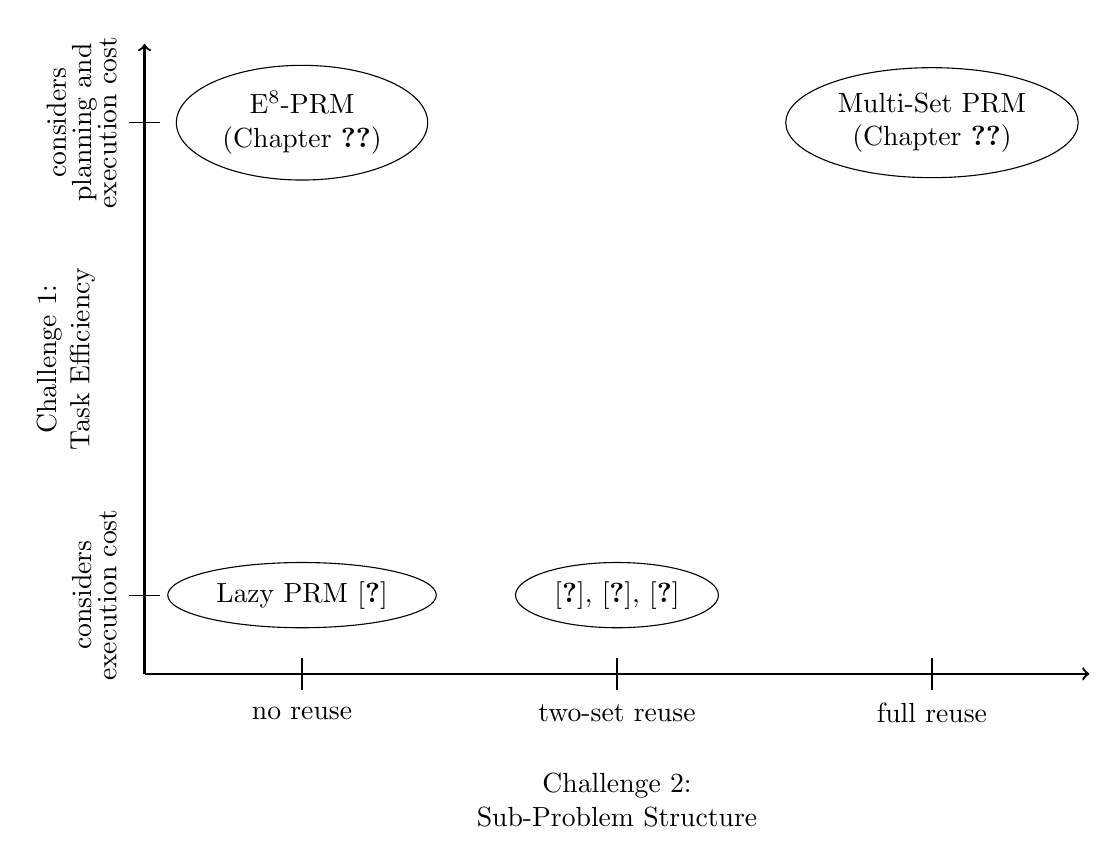
\begin{tikzpicture}

% axes
\draw[->,thick] (0,0) -- (0,8); 
\draw[->,thick] (0,0) -- (12,0);
\node[rotate=90,align=center] at (-1.0,4)
   {Challenge 1:\\Task Efficiency};
\node[align=center] at (6,-1.6)
   {Challenge 2:\\Sub-Problem Structure};

% y tics
\draw (-0.2,1) -- (0.2,1);
\node[rotate=90,align=center] at (-0.64,1)
   {considers\\[-0.04in]execution cost};
\draw (-0.2,7) -- (0.2,7);
\node[rotate=90,align=center] at (-0.8,7)
   {considers\\[-0.04in]planning and\\[-0.04in]execution cost};

% x tics
\draw (2,-0.2) -- (2,0.2);
\node[align=center] at (2,-0.5) {no reuse};
\draw (6,-0.2) -- (6,0.2);
\node[align=center] at (6,-0.5) {two-set reuse};
\draw (10,-0.2) -- (10,0.2);
\node[align=center] at (10,-0.5) {full reuse};

% algorithms
\node[draw,ellipse,align=center] at (2,1)
   {Lazy PRM \cite{bohlin2000lazyprm}};

\node[draw,ellipse,align=center] at (6,1)
   {\cite{leven2000changing}, \cite{kallman2004dynamicroadmaps},
   \cite{jaillet2004dynamicprm}};

\node[draw,ellipse,align=center] at (2,7)
   {E$^8$-PRM\\(Chapter~\ref{chap:inflate})};

\node[draw,ellipse,align=center] at (10,7)
   {Multi-Set PRM\\(Chapter~\ref{chap:multi-set-prm})};

\end{tikzpicture}
\caption{Graphical outline of $\mathcal{C}$-space planners.
   Work in progress.}
\label{fig:graphical-outline}
\end{center}
\end{widepage}
\end{figure}
}

%\begin{figure}
%\begin{widepage}
%   \centering
%   \begin{subfigure}[b]{0.24\textwidth}
%      \begin{center}
%      \includegraphics[width=\textwidth]{figs/switchboard.jpg}
%      
%      \includegraphics[width=\textwidth]{figs/mech-switches.jpg}
%      \end{center}
%      \caption{Something}
%   \end{subfigure}
%   \begin{subfigure}[b]{0.24\textwidth}
%      \begin{center}
%      \includegraphics[width=\textwidth]{figs/assembly-line.jpg}
%      
%      \includegraphics[width=\textwidth]{figs/car-robots.jpg}
%      \end{center}
%      \caption{Something}
%   \end{subfigure}
%   \begin{subfigure}[b]{0.24\textwidth}
%      \begin{center}
%      \includegraphics[width=\textwidth]{figs/table-clearing.jpg}
%      
%      \includegraphics[height=2in]{figs/herb-fuze.jpg}
%      \end{center}
%      \caption{HERB Robot}
%   \end{subfigure}
%   \begin{subfigure}[b]{0.24\textwidth}
%      \begin{center}
%      \includegraphics[width=\textwidth]{figs/chernobyl.jpg}
%      
%      \includegraphics[height=2in]{figs/chimp-debris.jpg}
%      \end{center}
%      \caption{CHIMP Robot}
%   \end{subfigure}
%   \caption{Manipulation problems.}
%\end{widepage}
%\end{figure}

\chapter{Framework for Efficient Manipulation Task Planning}
\label{chap:proposal-framework}

\begin{figure*}
   \begin{center}
   
   \subfloat[Start config]{%
      \includegraphics[width=0.19\linewidth]{figs/testherb-a.png}%
   }
   \,
   \subfloat[Step 1 in $X_1$]{%
      \includegraphics[width=0.19\linewidth]{figs/testherb-b.png}%
   }
   \,
   \subfloat[Step 2 in $X_2$]{%
      \includegraphics[width=0.19\linewidth]{figs/testherb-c.png}%
   }
   \,
   \subfloat[Step 3 in $X_3$]{%
      \includegraphics[width=0.19\linewidth]{figs/testherb-d.png}%
   }
   \,
   \subfloat[End config]{%
      \includegraphics[width=0.19\linewidth]{figs/testherb-e.png}%
   }
   
   \subfloat{
      \includegraphics{build/diagram-multi-step}
   }

   \caption[][99in]{x}
   \label{fig:xx-diagram-multi-step}

   \end{center}
   
   \smallskip\noindent\small Figure \ref{fig:xx-diagram-multi-step}:
      Diagram of multi-step planning framework.
      This thesis focuses on efficient geometric planning
      for manipulation tasks (the lower two levels here).
      Task planning can be performed by an autonomous
      symbolic planner,
      or guided by a human operator.
\end{figure*}

This chapter lays out our proposed approach
to planning for coupled manipulation tasks.
The reader is directed to
Figure~\ref{fig:xx-diagram-multi-step}
%Figure~2.1
for an overview.
Our approach consists generally of decomposing the task into
multiple steps,
each of which is solved by queries to an underlying motion
planner in the robot's
\emph{configuration space}\cite{lozanoperez1983cspace}.

% from sidd:
%Where to steps come from?
%what do i mean by steps?
%what is a step?
%walking, parkour
%cosntrained door opening
%reaching into a box
%replacing the car tire
%we focus on manipuation
%opening a door are manipuation
%two things that produce structure:
%- cobs
%- cspace manifolds
%we're just looking at a projection of the composite c-space

We suggest that a reasonable decomposition of a task into steps
should be guided by changes to either
the valid subset of the robot's configuration space
(e.g. at grasp and release points of manipulated objects)
or the set of constraints active on the robot's configuration.
This facilitates simpler calls to each motion planner,
and also allows separate planners with different capabilities
(e.g. constrained planners)
to be used for each step.

\paragraph{Outline.}
Loosely, the sections in this chapter are layed out as follows.
Sections~\ref{chap:e8} and~\ref{chap:graphs-in-continuous}
describe our approach to planning \emph{within} each step,
on graphs and roadmaps respectively.
Next,
Sections~\ref{chap:multi-set} and~\ref{chap:multi-set-prm}
identify and exploit structure \emph{between} steps
in order to reuse planning computation across queries.
Lastly,
Sections~\ref{chap:cmr} and~\ref{chap:task-planning}
discuss how to specify queries across all steps
in a higher-level sequencing task planner.


\clearpage
\section{Quickly Searching Explicit Expensive Graphs}
\label{chap:e8}

In order for a robot to perform manipulation tasks
in changing, unstructured environments,
it must be able to quickly solve planning queries.
In this section,
we discuss formulating
the motion planning problem as best-first graph search over paths
and propose an algorithm on explicit graphs.
Our approach is motivated by two insights.

\paragraph{Explicit Optimization of Ensemble Effort.}
This section reference two different types of efficiency
with regard to robotic tasks.
First, once a planner has computed a solution path or trajectory,
there is the cost incurred while executing that trajectory.
This is the traditional cost optimized for by planners.
Second, there is the cost incurred from actually computing the solution
itself.
We propose to optimize for both types of effort explicitly.

\paragraph{Explicit Graph Representation.}
We contend that representing graphs explicitly
is better suited to search over roadmap graphs
for two reasons.
First, it is reasonable to store the entire graph
\emph{explicitly} in memory
(e.g. ~10k vertices for a 7-DOF arm);
techniques to incrementally build the graph
via an implicit graph representation
are not necessary.
Second,
it is evaluating edge costs
(as opposed to expanding vertices or maintaining
a sorted open list)
that dominates planning costs.
In other words,
precious planning effort is principally manifested in
\emph{evaluated edge costs},
not \emph{determined vertex $g$-values}.

\subsection{Generic Best-First Search Algorithm over Paths}

Best-first search\cite{winston1977ai}
is a general class of search algorithms.
We choose to express the general algorith
over \emph{paths} instead of \emph{vertices}
for clarity and generality
because we are focused primarily on explicit graphs.
%See Algorithm~\ref{alg:generic-best-first}.
\begin{algorithm}
   \caption{Generic Best-First Search Algorithm Outline}
   \label{alg:generic-best-first}
   \begin{algorithmic}[1]
   \Procedure {\textsc{GenericBestFirst}}{$G$}
   \Loop
      \State $\pi^* = \argmin\limits_{\pi \in \Pi} f(\pi)$
         \Comment{For some path cost function $f(\pi)$}
         \label{line:generic-select-optimistic-path}
      \If {$\pi^*$ fully evaluated}
         \State \Return $\pi^*$
      \EndIf
      \State \textsc{EvalPath}$(\pi^*)$
         \Comment{For some evaluation function}
   \EndLoop
   \EndProcedure
   \end{algorithmic}
\end{algorithm}

\noindent
This formulation admits two choices:

\paragraph{Cost Function $f(\pi)$.}
What is the cost function $f(\pi)$ over paths used to select the
path for evaluation at each iteration?
Traditional graph search uses the following path objective:
\begin{equation}
   f(\pi) = \hat{f}_x(\pi): \mbox{\emph{optimistic estimate of execution effort}}.
\end{equation}
In other worts, $\hat{f}_x(\pi)$
gives a lower bound on the cost of executing
path $\pi$
given the algorith's current knowledge of the graph.
In our case,
if the path consists of a mix of evaluated and unevaluated edges,
we could write this as:
\begin{equation}
   \hat{f}_x(\pi) = \sum_{e \in \pi} \left\{
   \begin{array}{cl}
      x[e] & \mbox{if edge } e \mbox{ evaluated}  \\
      \hat{x}(e) & \mbox{otherwise} \\
   \end{array}
   \right.
   ,
   \label{eqn:execution-cost-objective}
\end{equation}
with $\hat{x}(e)$ an admissible estimate of the edge's execution effort.

\paragraph{Evaluation Procedure $\mbox{\sc EvalPath}(\pi)$}.
How is a potential path evaluated?
We discuss this later in this section.

\vspace{0.1in}
The choice of these two components of the algorithm
intimately depend on the graph representation.
For appropriate selection
of $f(\pi)$ and \textsc{EvalPath},
traditional algorithms such as A* \citep{hart1968astar}
and the Bidirectional Heuristic Front-to-Front Algorithm
\citep{sint1977bhffa}
are instances of this general formulation.

\subsection{Penalizing Planning Effort}

So far, we've been searching for a path which optimizes our execution
effort objective (\ref{eqn:execution-cost-objective}).
However, as we motivated earlier,
there are two distint notions of efficency;
here, we focus instead on \emph{planning efficiency}.
Consider the following path objective:
\begin{equation}
   f(\pi) = \hat{f}_p(\pi) : \mbox{\emph{optimistic estimate of planning effort}}.
\end{equation}

For problems over large graphs,
planning effort may be dominated by discovering vertex successors
or maintaining a sorted vertex open list.
\marginnote{Traditional metrics for planning
effort include \emph{vertiex expansions}
and \emph{heap percolates}.}
However, in many manipulation problems,
planning effort is instead dominated by \emph{edge evaluations}.
Therefore, our objective $\hat{f}_p$
penalizes remaining effort required to evaluate edges
along a path:
\begin{equation}
   \hat{f}_p(\pi) = \sum_{e \in \pi} \left\{
   \begin{array}{cl}
      0 & \mbox{if edge } e \mbox{ evaluated}  \\
      \hat{p}(e) & \mbox{otherwise} \\
   \end{array}
   \right.
   .
\end{equation}
The new edge heuristic $\hat{p}(e)$ estimates this evaluation cost.
\marginnote{Suggested metrics for $\hat{p}$
   include planning time or computational energy.}

The first graph planner to explicitly include such a heuristic
to estimate the remaining
computational planning effort in a best-first search
was A$_\epsilon^*$ \citep{pearl1982semiadmissible}.
While the approach we take is different,
a motivating quote from this paper is relevant:
\begin{quote}
``The heuristic [\,$\hat{x}$\,] ... is of an entirely
different nature than the ... heuristic [\,$\hat{p}$\,] ... .
The former anticipates the reduction in \emph{solution quality} due to the
remaining part of the solution once it is found;
the latter estimates the \emph{computational effort}
required for completing the search.''
\end{quote}

\subsection{Ensemble Effort Objective}

In general, we might consider weighting each objective:
\begin{equation}
   f(\pi) = \lambda \hat{f}_p(\pi) + (1 - \lambda) \hat{f}_x(\pi) .
   \label{eqn:general-objective}
\end{equation}
We call this effort model
\emph{ensemble effort}
in that it combines both planning and execution effort.
Note that with $\lambda=0$,
we recover our old solution cost objective $\hat{f}_x(\pi)$.
%Note that this objective is used in an optimistic, greedy fashion at each
%iteration of best-first search.
Represented over edges,
we can write:
\begin{equation}
   f(\pi) = \sum_{e \in \pi} \left\{
   \begin{array}{cl}
      (1 - \lambda) x[e] & \mbox{if edge } e \mbox{ evaluated}  \\
      \lambda \hat{p}(e) + (1 - \lambda) \hat{x}(e) & \mbox{otherwise} \\
   \end{array}
   \right.
   .
   \label{eqn:general-objective-explicit}
\end{equation}
We represent a particular choice of $\hat{p}(e)$
and $\hat{x}(e)$,
along with the evaluation function $x(e)$,
as an \emph{ensemble effort model}
denoted with $\mathcal{M}$:
\marginnote{For examples of ensemble effort models,
see Section~\ref{subsec:ensemble-effort-models}.}
\begin{equation}
   \mathcal{M} : (x, \hat{x}, \hat{p})
\end{equation}

\paragraph{Simplification with Propotional Heuristics.}

Suppose that our heuristic for planning effort
were proportional to that for execution effort,
\begin{equation}
   \hat{p}(e) = \alpha \, \hat{x}(e) .
\end{equation}
\marginnote{%
This might happen if, for example, each were proportional to the edge's
\emph{distance} (with longer paths taking longer to both collision check
and execute at constant velocity).}%
In this case, we can write:
\begin{equation}
   f(\pi) = (1-\lambda) \sum_{e \in \pi} \left\{
   \begin{array}{cl}
      x[e] & \mbox{if edge } e \mbox{ evaluated}  \\
      \left[ 1 + \frac{\alpha\lambda}{1 - \lambda} \right] \hat{x}(e) & \mbox{otherwise} \\
   \end{array}
   \right.
   .
   \label{eqn:prop-heuristics}
\end{equation}
Further,
if we use an \textsc{EvalPath}() function which forward-evaluates
vertices or edges
(as is required with implicit graph representations),
and $\lambda < 1$,
we can rewrite (\ref{eqn:prop-heuristics}) as:
\begin{equation}
   f(\pi) \propto
   \underbrace{\sum_{e \; \mbox{\scriptsize evaled}} x[e]}_{g[v_f]}
   +
   \underbrace{\left[ 1 + \frac{\alpha \lambda}{1-\lambda} \right]}_{
      \mbox{\scriptsize inflation factor } \epsilon}
   \underbrace{\hat{x}(e_{last})}_{h(v_f)}
   .
\end{equation}

In other words,
\emph{weighted A* is equivalent to
   best-first search whose objective
   includes a planning effort term
   proportional to execution effot.}
In particular, if planning effort is proportional to execution
effort by a factor of $\alpha$,
a weighted A* search with inflation factor $\epsilon$
is the result of best-first search with
$\lambda = \frac{\epsilon-1}{\alpha+\epsilon-1}$.

\subsection{The E$^8$ Explicit Graph Search Algorithm}
\label{sec:e8-planner}

The E$^8$ algorithm
(Exploiting Ensemble Effort Estimates
on Explicit graphs with Expensive Edge Evaluations)
is the result of applying
best-first search with the $\lambda$-mediated objective
from (\ref{eqn:general-objective}).
The algorithm is \emph{lazy},
in that edge evaluations are deferred until they are needed.
In fact, it can be seen as a generalization of the
LazyPRM \citep{bohlin2000lazyprm},
but which also considers planning effort in its objective.
Further,
the algorithm is \emph{heuristic-focused},
guided by its cost model $\mathcal{M}$.
Its behavior mimics that of an inflated heuristic planner
depending on the selection of the planning/execution cost
tradeoff parameter $\lambda$.

\begin{algorithm}[t]
\caption{E$^8$ Explicit Graph Search}
\label{alg:e8}
\begin{algorithmic}[1]
   \Procedure {E$^8$}{$G,
      V_{\mbox{\scriptsize start}}, V_{\mbox{\scriptsize goal}},
      \mathcal{M}, \lambda$}
   \State $x_{\mbox{\scriptsize eval}}[\cdot] \leftarrow$ empty map
      ($x_{\mbox{\scriptsize eval}} : E \rightarrow \mathbb{R}_0^+$)
      \label{line:store-edge-eval-efforts}
   \ForAll {$e \in G$}
      \State $e.{\mbox{cost}} \leftarrow
         \lambda \, \hat{p}(e) + (1 - \lambda) \, \hat{x}(e)$
         \Comment Ensemble effort model $\mathcal{M}$
         \label{line:edge-cost}
   \EndFor
   \Loop
         \label{line:best-first-start}
      \State $\pi^* = \mbox{\sc BiDijkstras}(G,
         V_{\mbox{\scriptsize start}}, V_{\mbox{\scriptsize goal}})$
         \label{line:e8-select-optimistic-path}
      \If {$e \in x_{\mbox{\scriptsize eval}} \;\forall\; e \in \pi^*$}
         \State \Return $\pi^*$
            \label{line:return-done}
      \EndIf
      \State $E_{\mbox{\scriptsize to\_eval}} \leftarrow
         \mbox{\sc PathEvalOrder}(\pi^*)$
         \Comment{See Section \ref{subsec:alg-path-evaluation}}
         \label{line:path-eval-order}
      \ForAll {$e \in E_{\mbox{\scriptsize to\_eval}}$}
         \State $x_{\mbox{\scriptsize eval}}[e] \leftarrow x(e)$
            \Comment Evaluate edge (expensive!)
            \label{line:evaulate-edge}
         \State $e.{\mbox{cost}} \leftarrow
            (1 - \lambda) \, x_{\mbox{\scriptsize eval}}[e]$
            \Comment Update ensemble estimate
            \label{line:update-estimate}
         \If {$x_{\mbox{\scriptsize eval}}[e] > \hat{x}(e)$}
            \label{line:exec-cost-check}
            \State \textbf{break}
               \label{line:eval-break}
         \EndIf
      \EndFor
   \EndLoop
      \label{line:best-first-end}
   \EndProcedure
\end{algorithmic}
\end{algorithm}

The E$^8$ algorithm (Algorithm~\ref{alg:e8})
directly follows the outline
of best-first search over paths
(Algorithm~\ref{alg:generic-best-first}).
Since edge evaluations are expensive,
we maintain a map $x_{\mbox{\scriptsize eval}}[\cdot]$
storing the known execution costs of all edges evaluated so far
(line~\ref{line:store-edge-eval-efforts}).
Each edge's current cost (line~\ref{line:edge-cost})
is derived from the problem's ensemble effort model $\mathcal{M}$.

At each iteration,
we optimistically select the best path $\pi^*$
which minimizes the this ensemble objective.
We select over all paths which connect
a vertex in $V_{\mbox{\scriptsize start}}$
to a vertex in $V_{\mbox{\scriptsize goal}}$
(any-to-any).
\marginnote{For types of planner specifications besides
any-to-any, see Chapter~\ref{chap:cmr}.}

If this path is already fully evaluated,
we finish on line~\ref{line:return-done}.
Note that if edge costs $x(e)$ may be infinity
(e.g. to denote an infeasible edge),
the algorithm will terminate with a fully evaluated path
with infinite cost if no feasible path exists.

Otherwise,
we evaluate the path's unevaluated edges
(lines \ref{line:path-eval-order}
to \ref{line:eval-break}).
We do this in a particular order,
as discussed later in this section.
For each edge,
we evaluate its execution cost $x(e)$ (line~\ref{line:evaulate-edge})
and update our effort estimate (line~\ref{line:update-estimate})
to account for (a) the actual execution effort
and (b) the fact that no additional planning effort is needed.
If the execution cost of any edge of the path proves
more expensive than we had anticipated
(line~\ref{line:exec-cost-check}),
we break and select a new path.

The E$^8$ algorithm admits a number of choices.

\paragraph{Choosing $\lambda$.}
The choice of the $\lambda$ parameter
affects the algorithm's tradeoff between planning and execution effort.
\marginnote{See research question \ref{ques:choosing-lambda}.}

\paragraph{Finding the Optimistic-Optimal Path.}
The current implementation of E$^8$ uses
bidirectional Dijkstra's algorithm
(line~\ref{line:e8-select-optimistic-path})
to select the lowest-cost path through the graph
at each iteration of the algorithm.
However, since the cost of only a few edges
are adjusted at each iteration (line~\ref{line:update-estimate}),
it appears to be well-suited to incremental
graph search algorithms (e.g. \citep{koenig2004lpastar})
to improve search efficiency.
\marginnote{See research question \ref{ques:incremental-search}.}

\paragraph{Selecting the Edge Evaluation Order.}
\label{subsec:alg-path-evaluation}
Once a candidate path is selected,
its constituent unevaluated edges are evaluted
in a particular order (line~\ref{line:path-eval-order}).
Our current algorithm
orders the edges alternating from the ends in.
\cdnote{I need a figure to show this.}
With different choices (e.g. forwards or backwards),
E$^8$ looks a lot like A$^*$.
\marginnote{See research question \ref{ques:evalpath}.}

\subsection{Repeated Queries}

The E$^8$ algorithm is \emph{multi-query},
in that it maintains a data structure of evaluated edge
execution costs $x_{\mbox{\scriptsize eval}}[\cdot]$
which allows reuse between different planning problems
over the same graph $G$,
either sequentially or in interleaved fashion.
For different queries on the same graph,
edge evaluations can simply be used in subsequent searches.

When used in this fashion,
E$^8$ behaves similarily to Experience graphs%
\cite{phillips2012egraphs}.
E-graphs are a type of best-first search which
are designed to find paths quickly by incentivizing the planner
to rely on on edges from previous successful plans.
While the E-graph planner is originally expressed over implicit graphs,
we can instead express it explicitly
as in Algorithm~\ref{alg:generic-best-first}
with the following objective:
\begin{equation}
   f_{\mbox{\scriptsize E-graphs}}(\pi) \propto \sum_{e \in \pi} \left\{
   \begin{array}{cl}
      x[e] & \mbox{if edge } e \mbox{ evaluated, this search} \\
      \epsilon \, x[e] & \mbox{if edge } e \mbox{ evaluated, previous search} \\
     \epsilon \, \epsilon^E \, \hat{x}(e) & \mbox{otherwise} \\
   \end{array}
   \right.
\end{equation}

The E$^8$ algorithm
is therefore equivalent to a simplified version of the E-Graph algorithm
with $\epsilon=1$ and $\epsilon^E = 1 + \frac{\alpha \lambda}{1-\lambda}$,
with the exception that all evaluated edges are placed in the graph,
not just the edges on previous solution paths.
Note that E-graph shortcuts
are not necessary for small explicit graphs.

\subsection{Experimental Evaluation of the E$^8$ Algorithm}

We propose to perform experiments on graphs with
expensive edge evaluations
in order to evaluate the E$^8$ algorithm.
\marginnote{See research question \ref{ques:e8-comparisons}.}
See Figure~\ref{fig:e8-results} for an example problem.

\begin{figure}[t]
   \centering
   %\begin{center}
   
   % for stats
   \input{build/e8-world-astar-stats}
   \input{build/e8-world-wastar-stats}
   \input{build/e8-world-e8-stats}
   \subfloat[Planning world.]{
      \includegraphics{build/e8-world-intro}
   }
   \quad
   \subfloat[][A$^*$ search.\\
         Planning Effort: 692.3 \\ %\worldstatsastarplan\\
         Execution Effort: 14.2 %\worldstatsastarexec}
   ]{
      \includegraphics{build/e8-world-astar}
   }
   \vspace{0.05in}
   \subfloat[][Weighted A$^*$ search, $\epsilon=3$\\
         Planning Effort: 390.8 \\%\worldstatswastarplan\\
         Execution Effort: 18.5 %\worldstatswastarexec}
   ]{
      \includegraphics{build/e8-world-wastar}
   }
   \quad
   \subfloat[][E$^8$ search, $\lambda=0.5$\\
         Planning Effort: 358.8 \\%\worldstatseEplan\\
         Execution Effort: 20.5 %\worldstatseEexec}
   ]{
      \includegraphics{build/e8-world-e8}
   }
   
   \caption{A simple 2D explicit graph search problem,
      comparing three approaches.
      A robot (bottom left) must reach a goal position (top right)
      on an 8-connected graph
      while avoiding a wall (black).
      Execution effort is equal to path length.
      The planning effort required to check an edge is proportional
      to its distance to the blue radar at top.
      The E$^8$ algorithm's solution has a lower combined
      planning and execution effort.}
   \label{fig:e8-results}
\end{figure}

\clearpage
\section{Roadmaps in Continuous Spaces}
\label{chap:graphs-in-continuous}

This section explores how we can construct roadmaps covering
configuration space that can then be searched by the E$^8$ algorithm.
Here,
we focus on the single-query problem;
refer to Section~\ref{chap:multi-set}
for extension to cached data structures.
Due to this focus,
we strive to compare against alternative single-query approaches
as we discuss in Section~\ref{subsec:single-query-results}.

Although
our approach makes no commitment to the roadmap class
(e.g. probabalistic or lattice-based),
we propose to use Random Geometric Graphs (RGGs)
as roadmaps covering configuration space,
borrowing heavily from prior approaches \citep{kavrakietal1996prm}
and analyses \citep{karaman2011samplingoptimal}.
we make no commitment as to the connection strategy
(e.g. $r$-disk or $k$-nearest).
Note that by pre-computing a sequence of samples,
nearest-neighbor queries can be moved entirely offline.
Also,
since it can be computed offline,
you can sparsify it \citep{shaharabani2013sparsification}.

\subsection{Continuous-Space Problem Formulation}
\label{subsec:single-set-formulation}

Consider a planning problem in a configuration space $\mathcal{C}$
between start and goal configurations
within a collision-free subset
$\mathcal{C}_{\ms{free}} \subseteq \mathcal{C}$.
A continuous feasible solution path $q(t)$ must then satisfy
\begin{equation}
  \begin{array}{c}
  q(t) \in \mathcal{C}_{\ms{free}} \;\forall\; t \in [0,1] \\
  q(0) = q_{start},\; q(1) = q_{goal} . \\
  \end{array}
  \label{eqn:solution}
\end{equation}
Eqn. (\ref{eqn:solution})
specify single configurations
$q_{start}$ and $q_{goal}$,
but the formulation is trivially extended to start/goal sets.

While simple problems may admit explicit representations of
$\mathcal{C}_{\ms{free}}$,
recent approaches to complex problems
(e.g. sampling-based planners)
instead reason implicitly via test function(s).%
\cite{lavalle2006planningbook}
To capture this,
we endow $\mathcal{C}_{\ms{free}}$ with an
\emph{indicator function} $\mathbf{1}_{\ms{free}}(q)$:
\begin{equation}
  \mathbf{1}_{\ms{free}}(q) =
    \left\{ \begin{array}{ll}
      \mbox{True} & \mbox{if } q \in \mathcal{C}_{\ms{free}} \\
      \mbox{False} & \mbox{otherwise}.
    \end{array} \right.
  \label{eqn:indicator-function}
\end{equation}
The set itself can equivalently be defined w.r.t. its indicator:
\begin{equation}
  \mathcal{C}_{\ms{free}} =
  \{ q \in \mathcal{C} \;|\; \mathbf{1}_{\ms{free}}(q) = \mbox{True} \} .
\end{equation}
Common examples of such indicators
(\ref{eqn:indicator-function})
include validity checkers for
geometric (workspace) collision,
stability, and visibility constraints.
Note that for complex problems,
evaluation of these indicators 
tends to dominate planning effort.

Excusing the abuse of notation,
we define an analogous indicator functional
$\mathbf{1}_{\ms{free}}[\cdot]$
which operates on path segments $q(t)$.
We use parentheses for functions and brackets for functionals.
\begin{equation}
  \mathbf{1}_{\ms{free}}[q(t)] =
    \left\{ \begin{array}{ll}
      \mbox{True} & \mbox{if } q(t) \in \mathcal{C}_{\ms{free}}
         \;\forall\; t \in [0,1] \\
      \mbox{False} & \mbox{otherwise}.
    \end{array} \right.
  \label{eqn:single-indicator-functional}
\end{equation}
A common way to approximate this functional is to call the subset's
corresponding indicator function ${\bf 1}_{\ms{free}}(q)$
(e.g. a collision check) at some fixed resolution.

\subsection{Ensemble Effort Models}
\label{subsec:ensemble-effort-models}

The E$^8$ algorithm requires an ensemble effort model
$\mathcal{M}$ over graph edges.
Note that these models can be simply added element-wise.

\begin{genericfloat}
   {%
   \floatname{algorithm}{Alg.}% shorter captions
   \algrenewcommand\textproc{}% no smallcaps for procedures
   \begin{minipage}[t]{0.49\linewidth}%
      \vspace{-0.17in}%
      \begin{algorithm}[H]
         \caption{Set Validity Model
            $\mathcal{M}_{\ms{valid}}$}
         \label{alg:single-set-effort-model}
         \begin{algorithmic}[1]
         \Function {$x_{\ms{valid}}$}{$e, \mathcal{C}_{\ms{free}}$}
            \If {${\bf 1}_{\ms{free}}[q_e(t)]$}
               \State \Return $0$
            \Else
               \State \Return $\infty$
            \EndIf
         \EndFunction
         \Function {$\hat{x}_{\ms{valid}}$}{$e, \mathcal{C}_{\ms{free}}$}
            \State \Return $0$
         \EndFunction
         \Function {$\hat{p}_{\ms{valid}}$}{$e, \mathcal{C}_{\ms{free}}$}
            \State \Return $\hat{p}_{\ms{free}}[q_e(t)]$
         \EndFunction
         \end{algorithmic}
      \end{algorithm}
   \end{minipage}%
   \hspace{0.02\linewidth}%
   \begin{minipage}[t]{0.49\linewidth}%
      \vspace{-0.17in}%
      \begin{algorithm}[H]
         \caption{Distance Model
            $\mathcal{M}_{\ms{dist}}$}
         \label{alg:dist-effort-model}
         \begin{algorithmic}[1]
         \Function {$x_{\ms{valid}}$}{$e$}
            \State \Return $|| q_e(1) - q_e(0) ||$
         \EndFunction
         \Function {$\hat{x}_{\ms{valid}}$}{$e$}
            \State \Return $|| q_e(1) - q_e(0) ||$
         \EndFunction
         \Function {$\hat{p}_{\ms{valid}}$}{$e$}
            \State \Return $0$
         \EndFunction
         \end{algorithmic}
      \end{algorithm}
   \end{minipage}%
   }%
\end{genericfloat}

\paragraph{Models of Planning Effort.}
Suppose we also have an estimate $\hat{p}_{\ms{free}}[q(t)]$
of the effort required to evaluate the indicator functional
(\ref{eqn:single-indicator-functional}),
for example proportional to the number of collision checks required.
The simplest way to capture subset membership of an edge $e$
during the search
is to map the indicator and its planning effort estimate
to real-valued costs as described in
$\mathcal{M}_{\ms{valid}}$
(Algorithm~\ref{alg:single-set-effort-model}).
Here, invalid edges imply infinite execution effort.

\paragraph{Models of Execution Effort.}
The simplest model might simply compute Euclidean distances between
vertices
($\mathcal{M}_{\ms{dist}}$,
Algorithm~\ref{alg:dist-effort-model}),
although other models are possible
(see Table~\ref{table:exec-cost-models}).
When posed as a traditional graph search problem,
E$^8$ requires an additive effort models --
the cost of a path is the sum of the costs of its consituent edges.
However,
for many problems it may be advantageous to consider
non-additive models (e.g. total smoothed time),
especially for execution costs for fast motions.
Note that non-additive models
render the path search problem more difficult.

\begin{margintable}
   \centering
   \begin{tabular}{lc}
      \toprule
      Model & Additive? \\
      \midrule
      Path Length & Yes \\
      Bounded-Vel-Acc \citep{hauser2010smoothing} & Yes \\
      Smoothed & No \\
      \bottomrule
   \end{tabular}
   \vspace{0.1in}
   \caption{Execution cost models.
      Additive models admit efficient graph search methods
      when choosing optimistic paths for evaluation.}
   \label{table:exec-cost-models}
\end{margintable}

\subsection{The E$^8$-PRM with Hard Batching}

\begin{algorithm}
\caption{E$^8$-PRM Planner with Hard Batching}
\label{alg:e8-prm-hard}
\begin{algorithmic}[1]
\State $G \leftarrow \mbox{empty graph}$
\State $\mathcal{M} \leftarrow
   \mathcal{M}_{\ms{valid}}(\mathcal{C}_{\ms{free}})
   + \mathcal{M}_{\ms{exec}}$
\Procedure {E$^8$-PRM}{$G,
   V_{\mbox{\scriptsize start}}, V_{\mbox{\scriptsize goal}},
   N, \mathcal{M}, \lambda$}
%\State $\mathcal{M}_{\ms{both}} \leftarrow
%   \mathcal{M}_{\ms{exec}}
%   + \mathcal{M}_{\ms{valid}}(\mathcal{C}_{\ms{free}})$
%\State $G.E \leftarrow \emptyset$
\Loop
   \State \textsc{PrmAddSamples}($G,
      V_{\mbox{\scriptsize start}}, V_{\mbox{\scriptsize goal}},
      N$)
   \State $\pi^* \leftarrow \mbox{E}^8(G,
      V_{\mbox{\scriptsize start}}, V_{\mbox{\scriptsize goal}},
      \mathcal{M}, \lambda)$
      \Comment See Algorithm~\ref{alg:e8}
   \If {$\hat{x}(\pi^*) < \infty$}
      \Comment $\hat{x}(\cdot)$ from cost model $\mathcal{M}$
      \State \Return $\pi^*$
   \EndIf
\EndLoop
\EndProcedure
\end{algorithmic}
\end{algorithm}

The E$^8$-PRM (Algorithm~\ref{alg:e8-prm-hard})
operates on an initially empty persistent roadmap graph $G$.
Each vertex represents a configuration $q \in \mathcal{C}$,
and each edge represents a path $q(t)$ planned by a local planner.

The E$^8$-PRM proceeds in \emph{batches};
at the start of each batch,
the \textsc{PrmAddSamples} procedure adds
$N$ additional vertices to the graph sampled from $\mathcal{C}$
(including sampled start and goal configurations from
$V_{\mbox{\scriptsize start}}, V_{\mbox{\scriptsize goal}}$
if not yet present),
and edges are generated according to the PRM construction method.

With the exception of the path evaluation strategy
(see Section~\ref{subsec:prm-path-eval}),
the E$^8$-PRM with $\lambda = 0$
is equivalent to 
the Lazy PRM \citep{bohlin2000lazyprm}.
Figure~\ref{fig:bean} shows solution paths for a simple
2D path planning problem for various runs of the algorithm.

\begin{figure}
   \centering
   \subfloat[Paths with $\lambda = 0$]{
      \includegraphics[width=0.45\textwidth]
      {figs/timegreedy-bean-lambda-00.png}
   }
   \,
   \subfloat[Paths with $\lambda = 1$]{
      \includegraphics[width=0.45\textwidth]
      {figs/timegreedy-bean-lambda-10.png}
   }
   \caption{Examples of paths for a 2d problems
      for different values of $\lambda$.
      As $\lambda$ is increased,
      paths are longer, but are faster to find.}
   \label{fig:bean}
\end{figure}

\subsection{Optimization in Expectation}

The purpose of the incremental graph densification strategy
achieved by hard batching (Algorithm \ref{alg:e8-prm-hard})
is to account for spatial correlation
in $\mathcal{C}_{\mbox{\scriptsize free}}$.
We would like to motivate this more formally.

We propose to extend the E$^8$-PRM planner
to minimize ensemble effort \emph{in expection}
using a probabalistic model of $\mathcal{C}_{\mbox{\scriptsize free}}$.
Even if this is too expensive,
we can motivate the incremental densification idea,
with a graduated cost model
to approximate a probabalistic model
of the $\mathcal{C}$-space.
\marginnote{See research question \ref{ques:batching}.}

\subsection{Path Evaluation}
\label{subsec:prm-path-eval}

In order to use the E$^8$ algorithm,
we must provide an edge evaluation function $x(e)$.
For feasibility checks
(e.g. tested via collision checkers),
we approximate each edge check
by evaluating the corresponding validity checker
at a fixed resolution along the path.

More generally, however,
since the E$^8$-PRM plans in a continuous space,
we can actually implement more complex path tests,
such as the whole-path bisection test used in the
Lazy PRM.
\marginnote{See research question \ref{ques:evalpath}.}

\subsection{Experimental Evaluation of the E$^8$-PRM}
\label{subsec:single-query-results}

\begin{figure}
   \centering
   \subfloat[RRT Ext-Con, R=1]{
      \includegraphics[width=0.3\textwidth]{figs/compare-2d-rrtc1-rrtextcon-r1-s1.png}
   }
   \,
   \subfloat[RRT Con-Con, R=1]{
      \includegraphics[width=0.3\textwidth]{figs/compare-2d-rrtc1-rrtconcon-r1-s1.png}
   }
   \,
   \subfloat[E$^8$-PRM, $\lambda=0$]{
      \includegraphics[width=0.3\textwidth]{figs/compare-2d-rrtc1-checkmask-l00-s1.png}
   }
   
   \vspace{0.05in}
   
   \subfloat[RRT Ext-Con, R=6]{
      \includegraphics[width=0.3\textwidth]{figs/compare-2d-rrtc1-rrtextcon-r6-s1.png}
   }
   \,
   \subfloat[RRT Con-Con, R=6]{
      \includegraphics[width=0.3\textwidth]{figs/compare-2d-rrtc1-rrtconcon-r6-s1.png}
   }
   \,
   \subfloat[E$^8$-PRM, $\lambda=1$]{
      \includegraphics[width=0.3\textwidth]{figs/compare-2d-rrtc1-checkmask-l10-s1.png}
   }
   
   \vspace{0.05in}
   
   \subfloat[Plot of collision checks vs solution path cost for the
         different algorithms.]{
      \includegraphics[width=0.8\textwidth]{figs/compare-2d-rrtc1-medians.png}
   }
   
   \caption{Example runs with different planners,
      with the same sequence of samples.
      Note that E$^8$-PRM with $\lambda=0$ is equivalent to the Lazy PRM.
      Red dots show collision checks.}
   \label{fig:compare-2d-rrtc1-vis}
\end{figure}

%\begin{figure}
%   \centering
%   \includegraphics[width=0.8\textwidth]{figs/timegreedy-herbstep1-comparison-cdfs.png}
%   \caption{Comparison between different algorithms on a HERB problem.}
%   \label{fig:herb-comparison-cdfs}
%\end{figure}

I hope to show that the E$^8$-PRM is competitive with RRT-Connect
in terms of planning effort required to find a feasible path.

We will compare this approach to
single-query baseline approaches
such as the RRT \citep{kuffner2000rrtconnect},
EST \citep{hsu1997expansive},
SBL \citep{sanchezante2001sbl},
and Lazy PRM \citep{bohlin2000lazyprm},
approaches over lattices such as E-graphs,
as well as asymptotically-optimal planners such as
RRT* \citep{karaman2011samplingoptimal}
and BIT* \citep{gammell2015bitstar}.
Also compare briefly against trajectory optimization approaches,
though these are largely complementary.
For example, there's CHOMP \citep{zucker2013chomp}
and TrajOpt \citep{schulman2013trajopt}.
Defer discussion of caching to subsequent
sections.

See Figure~\ref{fig:compare-2d-rrtc1-vis}
%and \ref{fig:herb-comparison-cdfs}
for results on a simple 2D problem.

\clearpage
\section{The Multi-Set Planning Problem}
\label{chap:multi-set}

Motion planning approaches that build graphs
in the collision-free subset of
configuration space,
e.g. the
PRM \citep{kavrakietal1996prm}
and RRT \citep{lavallekuffner1999rrt},
have proven promising
for high-dimensional articulated robotics problems
in unstructured environments.
These approaches devote a large amount of computational effort
testing configurations and paths for collision,
and the resulting graph can then be reused
for other queries in the same collision-free subset.
The E$^8$-PRM,
introduced above in Section~\ref{chap:graphs-in-continuous},
is another such approach.

However,
for manipuation problems,
this subset of the robot's configuration space
is sensitive to the locations and shapes of
both people and objects in the environment,
as well as the robot itself.
In addition, it depends on the shape and pose of any object
grasped by the robot.
This makes it difficult not only to apply the results of prior
planning computation to the current problem,
but also to efficiently consider planned or hypothesized motions,
since we must reconstruct our graph from scratch whenever
the environment changes.
This is especially the case for
multi-step manipulation tasks that must be planned into the future.
%We want to continuously update our representation for detours.

A large body of prior work has focused on methods to
improve planning efficiency on manipulation problems.
We show that many of these approaches are
in fact special instances of a more general structure,
which we formulate as the \emph{multi-set planning problem}.

\subsection{Multi-Set Problem Formulation}
\label{sec:multi-set-formulation}

\begin{figure*}
   \begin{widepage}
   \begin{center}

   \subfloat[
      A two-part multi-set problem in $\mathcal{C}$,
      first between $q_1$ and $q_2$ through $X_{12}$,
      then between $q_2$ and $q_3$ through $X_{23}$.
      The two free subsets $X_{12}$ and $X_{23}$ are distinct
      but related.
   ]{
      \includegraphics{build/figstar-a}
   }%
   \quad%
   \subfloat[
      The free subsets are related via other underlying
      subsets of $\mathcal{C}$, with $X_{12}=A \cap B$
      and $X_{23}=A \cap C$.
      A planner solving the first part (from $q_1$ to $q_2$)
      has found paths in $X_{12}$.
   ]{
      \label{subfig:figstar-intersections}
      \includegraphics{build/figstar-b}
   }%
   \quad%
   \subfloat[
      Due to the set relations,
      a planner solving the second part
      (from $q_2$ to $q_3$ in $X_{23}$)
      can reuse any segment known to be in $X_{12}$
      by checking only for its membership in $C$.
   ]{
      \includegraphics{build/figstar-c}
   }

   \vspace{0.1in}

   \subfloat[
      A forklift in a parking lot ($q_1$)
      must retrieve an object ($q_2$)
      and reverse park ($q_3$).
      This two-part problem
      requires plans in distinct collision-free
      $\mathcal{C}$-subsets
      $X_{12}$ and $X_{23}$.
   ]{%
      \begin{tabular}{c}
      \includegraphics{build/example-2d-a} \\
      \includegraphics{build/example-2d-b} \\
      \includegraphics{build/example-2d-c} \\
      \end{tabular}%
      \label{subfig:figstar-manip-probdef}
   }%
   \quad%
   \subfloat[
      Sets $X_{12}$ and $X_{23}$ are subsets of
      the configuration space of the robot $\mathcal{C}=\mbox{SE}(2)$,
      and can be represented as intersections
      of underlying subsets $A$, $B$, and $C$
      as in \protect\subref{subfig:figstar-intersections}.
   ]{%
      \label{subfig:figstar-manip-spaces}
      \begin{tabular}{c}
      \includegraphics{build/example-2d-d} \\
      \includegraphics{build/example-2d-e} \\
      \includegraphics{build/example-2d-f} \\
      \end{tabular}%
   }%
   \quad%
   \subfloat[
      After planning a path from $q_1$ to $q_2$ (top),
      a planner can reuse a configuration in $X_{12}$ (middle)
      by checking only for its membership in subset $C$,
      resulting in plan reuse (bottom).
   ]{%
      \begin{tabular}{c}
      \includegraphics{build/example-2d-g} \\
      \includegraphics{build/example-2d-h} \\
      \includegraphics{build/example-2d-i} \\
      \end{tabular}%
   }

   \caption[][99in]{x}
   \label{fig:multi-set}

   \end{center}
   \end{widepage}
   
   \vspace{0.1in}
   \smallskip\noindent\small Figure \ref{fig:multi-set}:
   An illustration of a multi-set planning
   problem in a common configuration space $\mathcal{C}$.
   The problem definition generalizes to an artibrary number of
   configuration space subsets and set relations between them.
   When two queries in different subests are solved sequentially,
   a multi-set planner can reuse path segments less expensively.
   See Section~\ref{sec:in-manipulation} for examples in
   manipulation.

\end{figure*}

The multi-set planning problem is
a generalization of both the movers' problem
and the multi-query planning problem%
\cite{kavrakietal1996prm}.
The reader is referred to
Fig.~\ref{fig:multi-set}
for a general example,
as well as a simple instantiation on a 2D manipulation task.
%which is discussed in more detail in
%Section~\ref{subsec:multi-prm-example}.
The multi-set problem formulation
explicitly captures both planning and execution effort
and can therefore be used as an ensemble effort model
for use in the E$^8$-PRM planner across queries.

The multi-set planning problem is multi-query in
a fixed configuration space $\mathcal{C}$.
However, unlike related problems in which all
queries demand solution paths contained within a single common subset of
$\mathcal{C}$
(usually the set of collision-free configurations, denoted
$\mathcal{C}_{\mbox{\scriptsize free}}$),
the multi-set problem allows for the specification of
\emph{multiple} such $\mathcal{C}$-subsets
$\mathcal{S} = \{ A, B, \dots \}$.
Like $\mathcal{C}_{\mbox{\scriptsize free}}$,
each member of $\mathcal{S}$
is a subset of the common configuration space
(that is,
$X \subseteq \mathcal{C} \;\forall\; X \in \mathcal{S}$),
and each subset $X$ has its own indicator and planning estimator
${\bf 1}_X[\cdot]$ and $\hat{p}_X(\cdot)$
as in Section~\ref{subsec:single-set-formulation}.
For example,
in Fig.~\ref{fig:multi-set}\subref{subfig:figstar-manip-spaces},
$\mathcal{C}$-subset $B$
consists of configurations
free of collision between the robot and
the initial object pose.

The problem supports an arbitrary number of queries $\mathcal{U}$.
Each query $u$ demands a solution path through a \emph{single}
$\mathcal{C}$-subset $U \in \mathcal{S}$
(see Fig~\ref{fig:query-to-subset}):
\begin{equation}
  u : ( q_{start},\; q_{goal},\; U ) .
  \label{eqn:q}
\end{equation}

\begin{marginfigure}
   \centering
   \subfloat[Multi-query planning]{
      \includegraphics{build/query-to-subset-a}
   }
   \vspace{-0.05in}
   \subfloat[Multi-set planning]{
      \includegraphics{build/query-to-subset-b}
   }
   \vspace{0.1in}
   \caption{While queries in multi-query planning reference
     the same subset of $\mathcal{C}$,
     each multi-set query references one of a number of such sets.}
   \label{fig:query-to-subset}
\end{marginfigure}

\begin{marginfigure}
   \centering
   \subfloat[Containment relation]{
      \begin{tabular}{cc}
      \includegraphics{build/relations-inclusion} \\
      $A \subseteq B$ \\
      $\mathbf{1}_A \Rightarrow \mathbf{1}_B$ \\
      \end{tabular}
   }
   \vspace{-0.05in}
   \subfloat[Intersection relation]{
      \begin{tabular}{cc}
      \includegraphics{build/relations-intersection} \\
      $A = B \cap C$ \\
      $\mathbf{1}_B \wedge \mathbf{1}_C \Rightarrow \mathbf{1}_A$ \\
      \end{tabular}
   }
   \vspace{0.1in}
   \caption{Types of subset relations.
     Each relation can be expressed directly as set relations
     or equivalently as logical statements
     on the corresponding indicator functions
     $\mathbf{1}_X(\cdot)$.}
   \label{fig:relations}
\end{marginfigure}

Finally, the multi-set problem incudes a list of set relations
$\mathcal{R}$
between the $\mathcal{C}$-subsets in $\mathcal{S}$.
These can be expressed directly using set theoretic relations,
or equivalently as logical statements
on the corresponding indicator functions.
Common types of such relations
(containment and intersection)
are illustated in Fig.~\ref{fig:relations}.
Fig.~\ref{fig:multi-set} gives an example of intersection relations;
an example of containment is a padded (conservative)
robot model (see Section~\ref{subsec:broad-phase}).

Together, these four elements
(a configuration space $\mathcal{C}$,
subsets $\mathcal{S}$ each with endowed indicators,
a set of queries $\mathcal{U}$,
and a list of subset relations $\mathcal{R}$)
comprise a multi-set planning problem.

\paragraph{Example Problem.}
Consider the diagram from Fig.~\ref{fig:multi-set}.
$\mathcal{S}$ consists of five $\mathcal{C}$-subsets labeled
$A$, $B$, $C$, $X_{12}$, and $X_{23}$,
and we have two queries,
$u_{12}: (q_1, q_2, X_{12})$
and
$u_{23}: (q_2, q_3, X_{23})$.
$\mathcal{R}$ consists of the two relations
$X_{12} = A \cap B$ and $X_{23} = A \cap C$.
Suppose a cost model $\mathcal{M}$
wherein evaluating the indicator
$\mathbf{1}_A$ incurs cost 4,
evaluating $\mathbf{1}_B$ and $\mathbf{1}_C$ incurs cost 2,
and evaluating $\mathbf{1}_{X_{12}}$ and $\mathbf{1}_{X_{23}}$
incurs cost 6.
In the manipulation example in
Fig.~\ref{fig:multi-set}\subref{subfig:figstar-manip-probdef},
this would be the case if each
pairwise outlined shape collision check incurs unit cost.

Suppose a graph structure within ${X_{12}}$ has been grown to solve
the first query $u_{12}$.
During the subsequent solve of query $u_{23}$,
an existing path segment known to be in ${X_{12}}$ can be shown to
also be contained within ${X_{23}}$ by only evaluating $\mathbf{1}_C$.
In the manipulation example,
reusing an a configuration from the previous search
would require only a check of cost 2,
instead of cost 6 for a new configuration.
Thus, we might hope that a planner may be biased towards reusing
said path segments in this case.

\subsection{Multi-Set Problems in Manipulation Tasks}
\label{sec:in-manipulation}

Instances of multi-set problems are especially prevalent when
planning for manipulation tasks with articulated robots.
This section details several such instances.
While these instances are discussed separately here,
they are often present simultaneously.
See Section~\ref{subsec:herb-experiment}
for experimental results for a problem
which includes several of the multi-set problem instances
described below.

We also provide an implementation for the
OpenRAVE \citep{diankov2010openrave}
virtual kinematic planning environment
which automatically discovers $\mathcal{C}$-subsets
in manipulation tasks.

\vspace{0.1in}
\noindent
%\textbf{Dynamic Environments}
\paragraph{Dynamic Environments.}
\label{subsec:dynamic-environments}

\begin{figure}
   \centering

   \begin{minipage}{.6\textwidth}
      \begin{tikzpicture}
      \tikzset{>=latex} % arrow heads
      \node[anchor=south west,inner sep=0] at (0,0)
        {\includegraphics[width=0.8\textwidth]{figs/chimp-voxels-delta.png}};

      \node[draw,inner sep=3pt,fill=white,fill opacity=0.9,align=center]
        (debrislab) at (0.7,1.0) {Debris object\\removed};
      \node[circle,inner sep=2,draw,fill=white] (debris) at (2.2,2.9) {};
      \draw[draw=black, double=white, double distance=1pt, line width=1pt]
        (debrislab.north) -- (debris);
        
      \node[draw,inner sep=3pt,fill=white,fill opacity=0.9,align=center]
        (addlab) at (5.0,2.0) {Additional\\voxels seen};
      \node[circle,inner sep=2,draw,fill=white] (added) at (4.4,5.0) {};
      \draw[draw=black, double=white, double distance=1pt, line width=1pt]
        (addlab.north) -- (added);
        
      \end{tikzpicture}
   \end{minipage}%
   \,%
   \begin{minipage}{.35 \textwidth}
      \includegraphics{build/retroactive-a}
      
      \includegraphics{build/retroactive-b}
   \end{minipage}

   \caption{
      Structured or unstructured dynamic environments
      can be represented as a multi-set problem
      (see Section~\ref{subsec:dynamic-environments}).
      
      \vspace{0.05in}
      \noindent
      (Left) A disaster response robot maintains a
      dynamic unstructured environment model
      using coarse voxels
      (scene data from a debris-clearing task at a
      recent disaster response competition).
      Since the last planning query,
      voxels have been added (green) and removed (red).
      
      \vspace{0.05in}
      \noindent
      (Right) $\mathcal{C}$-subsets and relations
      can be added retroactively.
      Here, the graph for an initial query is checked w.r.t $X_1$.
      After environment changes,
      $X_1$ is redefined in terms of the $\mathcal{C}$-subsets
      derived from the set of common, added, and removed elements,
      allowing for reuse on a query in $X_2$.
      Here,
      the planner need only check existing path segments
      against added voxels in order to reuse them for the current query.}
   \label{fig:dynamic-environments}
   %\label{fig:retroactive}
\end{figure}

The sensors on most articulated robots allow them to maintain
dynamic environment models to track changing collision geometry.
These models might be
structured (e.g. recognizing objects with known models)
or unstructured (e.g. occupancy models).
In both cases,
even in a changing world,
there are often areas that are fixed between planning queries.

Prior work (e.g. \citep{jaillet2004dynamicprm})
leverages this by imposing a dichotomy between
\emph{fixed} and \emph{moving} components of $\mathcal{C}$.
Our formulation extends this to an arbitrary number of such labels,
including ones defined retroactively (i.e. during planning;
see Fig.~\ref{fig:dynamic-environments}).
By explicitly labeling such areas in workspace
(and leveraging the \emph{set containment} property
\citep{newmanbranicky1991cspacetransforms}),
we can represent this structure as a multi-set planning problem.

\cdnote{%
Special case of this is if objects are disappearing.
Relation to occupancy grid representations of workspace
(for deltas, conservative approxs, etc).}

\paragraph{Grasped Objects}
\label{subsec:grasped-objects}

One instance specific to manipulation problems is the handling of
grasped objects.
For example, 
consider a manipulator which grasps a geometric object.
This affects the set of collision-free configurations
across a large section of $\mathcal{C}$
relative to the old set of valid configurations $X_{old}$.
However,
the resulting $\mathcal{C}$-subset $X_{new}$
can be represented simply as
$X_{new} = X_{old} \cap G$,
with $G$ the set of robot configurations in which
the \emph{grasped object} (only)
is deemed free of collision with the robot and environment.
This structure is discussed in the context of the
\emph{conditional reachability graph},
part of the \textsc{FFRob} heuristic framework
\citep{garrett2014ffrob}.

For example,
consider the manipulation problem in
Figure~\ref{fig:testherb-problem}.
The robot must find a path which moves its arm to grasp the cup.
After the cup is grasped,
the robot can reuse any edge in the existing roadmap
by simply checking the grasped cup
against the remainder of the environment.
This structure,
together with the approach to dynamic environments,
are included together in the experimental results
(Section~\ref{subsec:herb-experiment}).

\begin{marginfigure}
   \centering
   \includegraphics{build/self-collision}
   \caption{A roadmap is pre-computed in $R$,
      the subset of $\mathcal{C}$ consisting of configurations free
      of robot self-collision.
      Online, the planner must find a path that's also within $E$,
      the subset free of environment collision.
      When solving this query in $X = R \cap E$,
      the Multi-Set PRM automatically prefers potential paths with
      pre-computed edges (e.g. shown in grey)
      due to lower planning costs over alternatives with lower
      execution costs.}
   \label{fig:self-collision-example}
\end{marginfigure}

\paragraph{Cached Self-Collision-Checked Roadmaps}
\label{subsec:cached-self-valid}

Self-collision checking is a potentially expensive component to
articulated motion planning;
in contrast to environment checking,
it is fundamentally quadratic in the number of moving links.
Further, pairs of links to be checked
tend to be relatively close to each other,
reducing the effeciveness of broad-phase approaches.

Leven and Hutchinson \citep{leven2000changing}
introduced the concept of a pre-cached roadmap consisting of
configurations and paths already known to be valid w.r.t.
self-collision.
As a type of invariant in $\mathcal{C}$,
this can be seen as a particular instance of multi-set planning.
See Fig.~\ref{fig:self-collision-example}.

\begin{figure*}[b]
   \centering
   
   \subfloat[
      A single-set planner testing simply for membership in
      $\mathcal{C}_{\mbox{\scriptsize free}}$
      treats a collision validity checker as a
      ``black box.''
      Internally,
      modern checkers first employ an inexpensive broad-phase check
      using a low-dimensional conservative representation
      to quickly identify non-colliding bodies before
      resorting to an expensive narrow-phase check.
   ]{%
      \includegraphics{build/broadphase-single}%
   }%
   \quad%
   \subfloat[
      A multi-set planner can explicitly reason about the
      conservative nature of the broad-phase check.
      This allows it to defer some narrow phase checks
      (often indefinitely)
      and instead prefer paths that require fewer expensive checks.
   ]{%
      \includegraphics{build/broadphase-multi}%
   }
   
   \caption[][0.0in]{Collision validity checking is a commonly used
     indicator function.
     The multi-set formulation allows an intelligent planner to
     reach inside the checker's ``black box'' and reduce the number
     of costly narrow-phase checks.
     Resulting paths tend to be cheaper to compute and
     stay further from obstacles.}
   \label{fig:broad-phase}
\end{figure*}

\paragraph{Integration with Broad-Phase Collision Checking}
\label{subsec:broad-phase}

The multi-set formulation also enables motion planners to
reason directly about different robot or environment models.
For example, consider two geometric robot models,
one with high quality (e.g. from a CAD program),
and one hand-tuned ``padded'' model consisting of 
a small number of simple conservative bounding volumes.
The $\mathcal{C}$-subsets derived from these models
are related by $R_{padded} \subseteq R_{CAD}$.
Collision checkers currently use a similar approach internally
to speed up collision checks (see Fig.~\ref{fig:broad-phase}.
and Fig~\ref{fig:broad-phase-2d}).

%\subsubsection*{Conservative Bounding Volumes for Different Grasps}
%
%\subsubsection*{Conservative Bounding Volumes for Hypothesized Objects}
%
%There's a sweet ICRA paper here.
%
%\subsubsection*{Dual Arm Stuff}
%
%I think this is related.
%
%Check right arm against gian left side box, etc.
%
%\subsubsection*{Dimensionality Reduction}
%
%The Handey \cite{lozanoperez1987handey} robot
%assumed a box that contained the wrist links at a range of DOF values.
%
%\subsubsection*{Dual-Arm Stuff}
%
%This is very similar to dimensionality reduction.
%
%Loose coupling between arms.
%
%Separate roadmaps for each arm.
%
%Investigate this multi-set structure.


\clearpage
\section{Multi-Set as an Effort Model for Roadmap Planners}
\label{chap:multi-set-prm}

This section lays out how to leverage the multi-set formulation
as a planning effort model
for use in the E$^8$-PRM.
The resulting algorithm,
the Multi-Set PRM,
exploits the multi-set structure inherent in manipulation problems
by efficiently reuses planning computation between related queries.

\subsection{The Multi-Set PRM}

The Multi-Set PRM (Algorithm~\ref{alg:multi-set-prm}) is a simple
extension of the \mbox{E$^8$-PRM}
(Section~\ref{chap:graphs-in-continuous}).
They key differences are that
(a) it reasons about $\mathcal{C}$-subsets
using logical propositions,
and (b) it uses a multi-set ensemble effort model
$\mathcal{M}_{\ms{multi}}$ to capture relations
between these subsets.

\begin{algorithm}
\caption{Multi-Set PRM Planner}
\label{alg:multi-set-prm}
\begin{algorithmic}[1]
\State $G \leftarrow \mbox{empty graph}$
\State $P_{\ms{global}} \leftarrow
   \mbox{global propositions from\;} \mathcal{R}$
\Procedure {MultiSetPRM}{$G,
   V_{\ms{start}}, V_{\ms{goal}},
   U, N, \lambda$}
\State $\mathcal{M} \leftarrow
   \mathcal{M}_{\ms{valid}}(U)
   + \mathcal{M}_{\ms{exec}}$
\State \Return $\mbox{E}^8\mbox{-PRM}(G,
      V_{\ms{start}}, V_{\ms{goal}},
      \mathcal{M}, N, \lambda)$
      \Comment See Algorithm~\ref{alg:e8-prm-hard}.
\EndProcedure
\end{algorithmic}
\end{algorithm}

\paragraph{Set Relations as Logical Propositions.}
The planner represents the list of set relations $\mathcal{R}$
(Section~\ref{chap:multi-set})
specified in the multi-set problem formulation
as a set of \emph{logical propositions} $P_{\ms{global}}$
which are considered globally applicable.
For example,
the proposition $\mathbf{1}_A \Rightarrow \mathbf{1}_B$
follows from the relation $A \subseteq B$
(see Fig.~\ref{fig:relations}).
In addition,
each edge $e$ in the roadmap $G$ is augmented with an initially empty
set $e.P$ containing all additional edge-specific propositions
known to be true as a result of any indicator functions evaluated
over that edge.
For example,
if planner evaluated the indicator $\mathbf{1}_B[e]$
and it returned False,
the proposition $\lnot\mathbf{1}_B$ would be added to $e.P$.
Together, such sets of propositions can be used as \emph{premises}
as part of an \emph{argument} to demonstrate a \emph{conclusion};
a logical solver can then be used validate or invalidate the argument.
For example, an argument with these premises and conclusion
$\{ (\mathbf{1}_A \Rightarrow \mathbf{1}_B), (\lnot\mathbf{1}_B) \}
\Rightarrow (\lnot\mathbf{1}_A)$
can be shown to be valid.

\paragraph{A Multi-Set Ensemble Effort Model.}
The key to the Multi-Set PRM is the ensemble effort model
$\mathcal{M}_{\ms{multi}}$
(Algorithm~\ref{alg:multi-set-effort-model})
which allows for evaluation of an edge
as well as estimates of its planning and execution effort
in a way that takes advantage of multi-set structure.
The core of this model is the {\sc MultiOptCert} function
which takes as input an edge $q_e$,
a query $\mathcal{C}$-subset $U$,
and a set of known logical propositions $P_{\ms{known}}$
for that edge,
and as output produces an \emph{optimistic validation certificate}
consisting of subset indicators which if evaluated would
validate the membership of the edge in $U$ with lowest effort.

\begin{algorithm}
\caption{Multi-Set Validitiy Effort Model
   $\mathcal{M}_{\ms{multi}}$}
\label{alg:multi-set-effort-model}
{\algrenewcommand\textproc{}% Used to be \textsc
\begin{algorithmic}[1]
\Function {$x_{\ms{multi}}$}{$e, U$}
   \State $(\mathcal{S}_{\ms{cert}}, b_{\ms{cert}}, {\hat p}_{\ms{cert}})
      \leftarrow \mbox{\sc MultiOptCert}(q_e, U,
      P_{\ms{global}} \cup e.P_{\ms{eval}})$
   \ForAll {$X \in \mathcal{S}_{\ms{cert}}$}
      \State $b_{\ms{eval}} \leftarrow \mathbf{1}_X[q_e]$
      \State $\arraycolsep=2pt
         e.P_{\ms{eval}} \leftarrow e.P_{\ms{eval}} \cup
         \left\{\begin{array}{rl}
         \mathbf{1}_X & \mbox{if } b_{\ms{eval}} \\
         \lnot \mathbf{1}_X & \mbox{otherwise} \\
         \end{array}
         \right\}$
      \If {$b_{\ms{eval}} \neq b_{\ms{cert}}(X)$}
         \State \Return $\infty$
      \EndIf
   \EndFor
   \State \Return $0$
\EndFunction
\Function {$\hat{x}_{\ms{multi}}$}{$e, U$}
   \State \Return $0$
\EndFunction
\Function {$\hat{p}_{\ms{multi}}$}{$e, U$}
   \State $(\mathcal{S}_{\ms{cert}}, b_{\ms{cert}}, {\hat p}_{\ms{cert}})
      \leftarrow \mbox{\sc MultiOptCert}(q_e, U,
      P_{\ms{global}} \cup e.P_{\ms{eval}})$
   \State \Return ${\hat p}_{\ms{cert}}$
\EndFunction
\end{algorithmic}
} %textproc
\end{algorithm}

\paragraph{Calculating the Multi-Set Optimistic Certificate}
%The \textsc{MultiOptCert} function (Alg.~\ref{alg:opt-edge-plan})
%performs the core reasoning which exploits the relations in
%the multi-set problem.
The \textsc{MultiOptCert} function (Alg.~\ref{alg:opt-edge-plan})
is tasked with computing
the optimistically optimal set of indicator evaluations to perform
for the edge in order to validate its membership in the query
$\mathcal{C}$-subset $U$.
The function returns three elements:
(a) the set of $\mathcal{C}$-subsets
$\mathcal{S}_{\ms{cert}} \subseteq \mathcal{S}$
whose indicators are to be evaluated,
(b) a binary function $b_{\ms{res}}$
which provides the desired indicator result for each evaluation,
and (c) the total evaluation cost ${\hat p}_{\ms{cert}}$
given by the $\hat{p}_X[\cdot]$ functionals
(Section~\ref{sec:multi-set-formulation}).

\begin{algorithm}
\caption{Multi-Set Optimistic Certification}
\label{alg:opt-edge-plan}
\begin{algorithmic}[1]
\Function {MultiOptCert}{$q_e, U, P_{\ms{known}}$}
   \State $\mathcal{T}_{\ms{imply}} \leftarrow \emptyset$
   \ForAll {$\mathcal{S}_{\ms{cert}} \in \mathcal{P}(\mathcal{S})$}
         \label{line:power-set}
      \State ${\hat p}_{\ms{cert}} \leftarrow \sum_{X \in \mathcal{S}_{\ms{cert}}} \hat{p}_X[q_e]$
      \ForAll {$b_{\ms{res}} \mbox{ \textbf{s.t.} }
            b_{\ms{res}} : \mathcal{S}_{\ms{cert}} \rightarrow \{\mbox{True},\mbox{False}\}$}
            \label{line:all-binary-functions}
         \State $\arraycolsep=2pt
            P_{\ms{res}} \leftarrow
            \left\{\left. \begin{array}{rl}
            \mathbf{1}_X & \mbox{if } b_{\ms{res}}(X) \\
            \lnot \mathbf{1}_X & \mbox{otherwise} \\
            \end{array}
            \right|
            X \in \mathcal{S}_{\ms{cert}}
            \right\}$
         \If {$P_{\ms{known}} \cup P_{\ms{res}}
               \Rightarrow \mathbf{1}_U$ is valid}
            \State $\mathcal{T}_{\ms{imply}} \leftarrow
               \mathcal{T}_{\ms{imply}} \cup
               \{ (\mathcal{S}_{\ms{cert}}, b_{\ms{res}}, {\hat p}_{\ms{cert}}) \}$
         \EndIf
      \EndFor
   \EndFor
   \State \Return $(\mathcal{S}_{\ms{cert}}, b_{\ms{res}}, {\hat p}_{\ms{cert}})
      \in \mathcal{T}_{\ms{imply}}$
      with lowest ${\hat p}_{\ms{cert}}$
\EndFunction
\end{algorithmic}
\end{algorithm}

The function accumulates a set $\mathcal{T}_{\ms{imply}}$ of
valid certificates which would imply membership in $U$.
We proceed by considering all combinations of
available $\mathcal{C}$-subset indicators
$\mathcal{S}_{\ms{cert}}$ (line~\ref{line:power-set}).
For each set of evaluations,
we compute the planning effort ${\hat p}_{\ms{cert}}$
which would be required.
We then consider all possible outcomes for each indicator
by iterating over all functions $b_{\ms{res}}$ mapping
from $\mathcal{C}$-subset $X$ to binary values
(line~\ref{line:all-binary-functions}).
For each potential outcome $b_{\ms{res}}$,
we form the set of additional propositions $P_{\ms{res}}$,
and then use a propositional logic solver to determine whether
the aggregate premises imply membership
in the query $\mathcal{C}$-subset $U$.
If so, this certificate is added to $\mathcal{T}_{\ms{imply}}$,
and the lowest-effort certificate is returned.

\subsection{Behavior of the Multi-Set PRM}

See Figure~\ref{fig:broad-phase-2d}
for a simple example with integrated broad-phase collision checking
as described in Section~\ref{subsec:broad-phase}.

\begin{figure}
   \centering

   \subfloat[][
      $\lambda=0$, no broad phase.\\
      Median planning cost: 6650
   ]{
      \includegraphics[width=0.45\linewidth]{figs/paths-lambda0-norel.png}
   }
   \subfloat[][
      $\lambda=1$, no broad phase.\\
     Median planning cost: 4530
   ]{
      \includegraphics[width=0.45\linewidth]{figs/paths-lambda1-norel.png}
   }
   
   \subfloat[][
      $\lambda=0$, with broad phase.\\
      Median planning cost: 2122
   ]{
      \includegraphics[width=0.45\linewidth]{figs/paths-lambda0-wrel.png}
   }
   \subfloat[][
      $\lambda=1$, with broad phase.\\
      Median planning cost: 737
   ]{
      \includegraphics[width=0.45\linewidth]{figs/paths-lambda1-wrel.png}
   }

   \caption{A simple 2D example of the Multi-Set PRM using
     a broad-phase check.
     Checking for collision with the grey box is 10x less expensive
     than with the actual black obstacle.}
     %\cdnote{I need to talk about this in the text.}}
   \label{fig:broad-phase-2d}
\end{figure}

\subsection{Home Robot Manipulation Task Results}
\label{subsec:herb-experiment}

\begin{figure*}[t]
   \centering
   
   \subfloat[Starting Configuration]{
      \includegraphics[width=0.185\linewidth]{figs/testherb-a.png}
   }
   \subfloat[Step 1, in $X_1$]{
      \includegraphics[width=0.185\linewidth]{figs/testherb-b.png}
   }
   \subfloat[Step 2, in $X_2$]{
      \includegraphics[width=0.185\linewidth]{figs/testherb-c.png}
   }
   \subfloat[Step 3, in $X_3$]{
      \includegraphics[width=0.185\linewidth]{figs/testherb-d.png}
   }
   \subfloat[Ending Configuration.]{
      \includegraphics[width=0.185\linewidth]{figs/testherb-e.png}
   }

   \caption[][0.2in]{
     A home robot performing a three-step manipulation task.
     It must move from its home configuration
     to grasp the cup,
     transfer it to a drop location above the bin,
     and return home.
     Experimental results for the Multi-Set PRM
     are shown in Table~\ref{tab:testherb}}
   \label{fig:testherb-problem}
\end{figure*}

\begin{table*}[b]
   \begin{widepage}
   \centering
   \footnotesize
   \setlength{\tabcolsep}{3pt}
   \renewcommand{\arraystretch}{1.3}
   \begin{tabular}{|cc|r@{ }lr@{ }lr@{ }lr@{ }l|r@{ }lr@{ }lr@{ }lr@{ }l|r@{ }lr@{ }lr@{ }lr@{ }l|}
   \toprule
   \multirow{2}{*}{Relations} & \multirow{2}{*}{Cost}
     & \multicolumn{8}{c|}{$\lambda = 0$}
     & \multicolumn{8}{c|}{$\lambda = 0.5$}
     & \multicolumn{8}{c|}{$\lambda = 1$}
   \\
     &
     & Step & 1 & Step & 2 & Step & 3 & \multicolumn{2}{c|}{Total}
     & Step & 1 & Step & 2 & Step & 3 & \multicolumn{2}{c|}{Total}
     & Step & 1 & Step & 2 & Step & 3 & \multicolumn{2}{c|}{Total}
   \\ \midrule
   \multirow{2}{*}{None} & Plan
     &  6.16&s &  3.72&s &  2.38&s & 12.25&s
     &  5.52&s &  2.89&s &  2.12&s & 10.53&s
     &  3.39&s &  2.25&s &  2.12&s &  7.76&s
   \\
     & Exec
     & 14.22&rad &  8.51&rad &  4.23&rad & 26.97&rad
     & 15.07&rad & 10.60&rad &  4.23&rad & 29.89&rad
     & 15.07&rad & 10.60&rad &  4.23&rad & 29.89&rad
   \\ [1ex]
   Inter-Step & Plan
     &  6.40&s &  2.33&s &  0.86&s &  9.59&s
     &  5.40&s &  1.55&s &  0.91&s &  7.86&s
     &  3.38&s &  0.91&s &  0.30&s &  4.59&s
   \\
   (Sec.~\ref{subsec:dynamic-environments},~\ref{subsec:grasped-objects})
     & Exec
     & 14.22&rad &  8.51&rad &  4.23&rad & 26.97&rad
     & 15.07&rad & 12.21&rad &  4.23&rad & 31.51&rad
     & 15.07&rad & 12.21&rad &  7.11&rad & 34.40&rad
   \\ [1ex]
   Self-Checked & Plan*
     &  3.54&s &  2.23&s &  1.17&s & 6.94&s
     &  2.99&s &  1.77&s &  1.16&s & 5.92&s
     &  1.47&s &  1.22&s &  1.16&s & 3.85&s
   \\
   (Sec.~\ref{subsec:cached-self-valid}) & Exec
     & 14.22&rad &  8.51&rad &  4.23&rad & 26.96&rad
     & 14.22&rad & 10.06&rad &  4.23&rad & 28.51&rad
     & 14.22&rad & 10.60&rad &  4.23&rad & 29.05&rad
   \\ [1ex]
   \multirow{2}{*}{Both} & Plan*
     &  3.25&s &  1.79&s &  0.90&s & 5.94&s
     &  2.88&s &  1.55&s &  0.92&s & 5.35&s
     &  1.47&s &  1.88&s &  0.31&s & 3.66&s
   \\
     & Exec
     & 14.22&rad &  8.51&rad &  4.23&rad & 26.96&rad
     & 14.22&rad &  8.51&rad &  4.23&rad & 26.96&rad
     & 14.22&rad &  9.64&rad &  6.36&rad & 30.22&rad
   \\ 
   \bottomrule
   \end{tabular}
   \caption[][-0.1in]{Home robot manipulation task results.
     The entry with no relations and $\lambda=0$ is equivalent
     to the LazyPRM.}
   \label{tab:testherb}
   \end{widepage}
\end{table*}

We tested the Multi-Set PRM on the manipulation task
described in Fig.~\ref{fig:testherb-problem}.
We used the $r$-disk PRM construction rule with $r=2.0$ rad,
and a batch size of $N=1000$.
Planning times are measured on a Lenovo T430s laptop.
The planner was asked to solve each of the steps of the plan
sequentially.

We varied
(a) the planning vs. execution parameter $\lambda$
(see Section~\ref{sec:e8-planner}), and
(b) the subset relations provided to the planner
as described in Section~\ref{subsec:dynamic-environments}.
We measured the time required for planning (s)
and the length of the resulting solution resulting path (rad)
for each step of the task.

Note that the Multi-Set PRM,
with no relations specified and $\lambda=0$
reduces to the Lazy PRM.
As expected,
increasing $\lambda$ resulted in decreased planning times
but yielded longer paths.
Including more $\mathcal{C}$-subset relations
also significantly reduced planning times,
and had little effect on path lengths on this problem.
Note that the planning time results when using
the cached self-collision-checked roadmap, denoted by (*),
do not include the pre-computation time.

Note that including inter-step relations drastically
reduces planning times for subsequent steps.
We expect this trend would continue as more steps are included.
Also, note that when $\lambda=0$,
path length is unchanged as the number of set relations is
changed
-- this is because the paths that are selected for evaluation
by the algorithm are a function only of their (constant) lengths.

%\subsection{Other Experiments to Run}
%
%\begin{itemize}
%\item with/without inter-step relations
%\item with/without padding
%\item with/without self-checked cache
%\item with/without relations for changing worlds
%\item with/without conservative boxes for grabbed objects
%\item constraints:
%   \begin{itemize}
%   \item handle with separate planner
%   \item handle with relaxed constraint, followed by local optimizer
%   \end{itemize}
%\item run optimizer on paths occasionally and/or before executing
%\end{itemize}


\clearpage
\section{Comprehensive Multi-Root Planning}
\label{chap:cmr}

While the Multi-Set PRM
allows planning computation to be reused between queries
across steps of a manipulation task,
a higher-level task planner must still distribute these queries
in order to discover a low-cost path
through all of the task's steps
(see Figure~\ref{fig:xx-diagram-multi-step}).
The types of queries we have discussed so far
(using sets
$V_{\mbox{\scriptsize start}}$ and $V_{\mbox{\scriptsize goal}}$)
take an \emph{any-to-any} form
-- the planner will return a successful path which connects
from any start to any goal vertex.
However,
when planning in parallel for multiple steps,
a task planner instead requires a \emph{diverse} set of
paths.

\begin{figure}
   \centering
   \subfloat[A real-world problem.]{
      \includegraphics[width=0.55\linewidth]{figs/herb-drilling.png}
      \label{subfig:herb-picture}
   }
   \caption{A real-world problem.}
   \subfloat[Illustration.]{
      \resizebox{0.35\linewidth}{!}{
      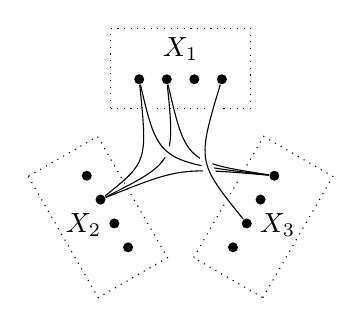
\begin{tikzpicture}[scale=0.7]

      \begin{scope}
      \node[rectangle,draw,dotted,
         inner sep=0,minimum height=0.4in,minimum width=0.7in] (x1) at (0,0) {};
      \node[below] at (x1.north) {$X_1$};
      \node[circle,inner sep=0,minimum size=0.05in,fill=black] (x1a) at (-0.75,-0.2) {};
      \node[circle,inner sep=0,minimum size=0.05in,fill=black] (x1b) at (-0.25,-0.2) {};
      \node[circle,inner sep=0,minimum size=0.05in,fill=black] (x1c) at ( 0.25,-0.2) {};
      \node[circle,inner sep=0,minimum size=0.05in,fill=black] (x1d) at ( 0.75,-0.2) {};
      \end{scope}

      \begin{scope}[shift={(-1.5,-2.7)},rotate=120]
      \node[rectangle,draw,dotted,rotate=120,
         inner sep=0,minimum height=0.4in,minimum width=0.7in] (x2) at (0,0) {};
      \node at (0,0.3) {$X_2$};
      \node[circle,inner sep=0,minimum size=0.05in,fill=black] (x2a) at (-0.75,-0.2) {};
      \node[circle,inner sep=0,minimum size=0.05in,fill=black] (x2b) at (-0.25,-0.2) {};
      \node[circle,inner sep=0,minimum size=0.05in,fill=black] (x2c) at ( 0.25,-0.2) {};
      \node[circle,inner sep=0,minimum size=0.05in,fill=black] (x2d) at ( 0.75,-0.2) {};
      \end{scope}

      \begin{scope}[shift={(1.5,-2.7)},rotate=-120]
      \node[rectangle,draw,dotted,rotate=-120,
         inner sep=0,minimum height=0.4in,minimum width=0.7in] (x3) at (0,0) {};
      \node at (0,0.3) {$X_3$};
      \node[circle,inner sep=0,minimum size=0.05in,fill=black] (x3a) at (-0.75,-0.2) {};
      \node[circle,inner sep=0,minimum size=0.05in,fill=black] (x3b) at (-0.25,-0.2) {};
      \node[circle,inner sep=0,minimum size=0.05in,fill=black] (x3c) at ( 0.25,-0.2) {};
      \node[circle,inner sep=0,minimum size=0.05in,fill=black] (x3d) at ( 0.75,-0.2) {};
      \end{scope}

      \draw (x1b) .. controls(-0.1,-1.7) .. (x2c);
      \draw[white,line width=4] (x1a) .. controls(-0.4,-1.7) .. (x3a);
      \draw (x1a) .. controls(-0.4,-1.7) .. (x3a);
      \draw (x1b) .. controls( 0.1,-1.7) .. (x3a);
      \draw (x1a) .. controls(-0.6,-1.7) .. (x2c);
      \draw (x3a) .. controls(0.0,-1.8) .. (x2c);
      \draw[white,line width=4] (x1d) .. controls( 0.3,-1.7) .. (x3c);
      \draw (x1d) .. controls( 0.3,-1.7) .. (x3c);

      \end{tikzpicture}
      }
      \label{subfig:cmr-illustration}
   }
   \caption{The comprehensive multi-root (CMR) problem.}
   \label{fig:cmr-problems}
\end{figure}

To handle this,
we formulate and study the
\emph{comprehensive multi-root} (CMR) planning problem
\cite{dellin2015cmr} (Figure~\ref{fig:cmr-problems}),
in which feasible paths are desired between multiple regions.
We propose two primary contributions which allow us to extend
state-of-the-art sampling-based planners.
First, we propose the notion of \emph{vertex coloring} as a compact
representation of the CMR objective on graphs.
Second, we propose a method for \emph{deferring edge evaluations}
which do not advance our objective, by way of a simple
criterion over these vertex colorings.
The resulting approach can be applied to any CMR-agnostic 
graph-based planner which evaluates a sequence of edges.
We prove that the theoretical performance of the colored algorithm
is always strictly better than (or equal to)
that of the corresponding uncolored version.
We then apply the approach to the Probabalistic RoadMap (PRM)
algorithm;
the resulting \emph{Colored Probabalistic RoadMap} (cPRM)
is illustrated on 2D and 7D CMR problems.

\subsection{The Comprehensive Multi-Root Problem}

We work with the robot's configuration space $\mathcal{C}$
and its collision-free subset $\mathcal{C}_{\mbox{\scriptsize free}}$.
We consider the general problem with $N$ root sets in this space
$\{ X_1, \dots, X_N \}$.
We seek a diverse set of feasible paths between root sets
-- that is, we want to maximize the number of connected roots between sets. 
We call this the \emph{comprehensive multi-root} (CMR) planning problem.

We track progress via the $r$-score:
\begin{equation}
   r = \big| \{
      \textsc{Path}(x_a,x_b) \;|\; x_a,x_b~\text{in different root sets}
      \} \big|.
   \label{eqn:obj}
\end{equation}
For example, the solution illustrated in
Figure~\ref{fig:cmr-problems}\subref{subfig:cmr-illustration}
has an $r$-score of 6 out of a maximum of 27.
Our objective is to \emph{maximize} the $r$-score as \emph{quickly} as
possible.

\subsection{A CMR Example}

\begin{figure*}[t]
   %\begin{widepage}
   \centering
   \begin{minipage}{.55\textwidth}
      \subfloat[PRM (86 Edges Checked) (195 Edges Considered, No Pairs)]{
         \includegraphics{build/w13-fu1-ec86}
         \label{subfig:w13-sameec-uncolored}
      }
      \subfloat[cPRM (86 Edges Checked) (344 Edges Considered, 1 Pair)]{
         \includegraphics{build/w13-fs1-ec86}
         \label{subfig:w13-sameec-colored}
      }
      \\ \quad \\
      \subfloat[PRM (344 Edges Considered) (125 Edges Checked, 8 Pairs)]{
         \includegraphics{build/w13-fu1-ei344}
         \label{subfig:w13-sameein-uncolored}
      }
      \subfloat[cPRM (344 Edges Considered) (91 Edges Checked, 8 Pairs)]{
         \includegraphics{build/w13-fs1-ei344}
         \label{subfig:w13-sameein-colored}
      }
   \end{minipage}
   \begin{minipage}{.43\textwidth}
      \subfloat[Edges considered, evaluated, deferred, and skipped.]{
         \includegraphics{build/plot-edges-w13}
         \label{subfig:w13-plot-edges}
      }
      \\ \quad \\
      \subfloat[CMR Objective vs edges evaluted.]{
         \begin{tikzpicture}[font=\scriptsize]
         % primary axis
         \begin{axis}[
            xlabel={Edges Checked},
            ylabel={Pairs Connected},
            %legend pos= north west,
            legend style={at={(axis cs:5,7.5)},anchor=north west},
            legend cell align=left,
            %axis equal image,
            width=3.4in,
            height=1.3in,
            xmin=0, xmax=150,
            %xmin=0, xmax=1000, ymin=0,
            %scaled ticks=base 10:-3,
            xlabel near ticks,
            ylabel near ticks]
         \addplot[black,ultra thick] table[col sep=space] {figs/w13-fu1-qs-pvc.txt};
         \addlegendentry{Uncolored}
         \addplot[mark=*,black,only marks,mark size=1,forget plot] plot coordinates {
            (125,8) % uc
         };
         \addplot[green,thick] table[col sep=space] {figs/w13-fs1-qs-pvc.txt};
         \addlegendentry{Colored}
         \addplot[mark=*,black,only marks,mark size=1,forget plot] plot coordinates {
            (86,1) %+1
            (87,2) %+1
            (89,4) %+2
            (90,6) %+2
            (91,8) %+2
         };
         \addplot[blue,mark=o,mark size=2] plot coordinates {(86,0) (86,1)}; % a-b comparison
         \addplot[blue,mark=o,mark size=2] plot coordinates {(125,8) (91,8)}; % c-d comparison
         % coordinates
         \coordinate (subfig_a_point) at (axis cs: 86,0);
         \coordinate (subfig_b_point) at (axis cs: 86,1);
         \coordinate (subfig_c_point) at (axis cs: 125,8);
         \coordinate (subfig_d_point) at (axis cs: 91,8);
         \end{axis}
         % labels
         \node[circle,inner sep=0pt,color=blue,fill=white] (subfig_b_label) at (2.9,0.6) {(b)};
         \node[circle,inner sep=0pt,color=blue,fill=white] (subfig_d_label) at (3.1,1.3) {(d)};
         \node[circle,inner sep=0pt,color=blue,fill=white] (subfig_a_label) at (4.9,0.5) {(a)};
         \node[circle,inner sep=0pt,color=blue,fill=white] (subfig_c_label) at (5.2,1.2) {(c)};
         \draw[color=blue,->] (subfig_b_label) -- ($ (subfig_b_point)!4pt!(subfig_b_label) $);
         \draw[color=blue,->] (subfig_d_label) -- ($ (subfig_d_point)!4pt!(subfig_d_label) $);
         \draw[color=blue,->] (subfig_a_label) -- ($ (subfig_a_point)!4pt!(subfig_a_label) $);
         \draw[color=blue,->] (subfig_c_label) -- ($ (subfig_c_point)!4pt!(subfig_c_label) $);
         \end{tikzpicture}
         \label{subfig:w13-plot-pairs}
      }
   \end{minipage}
   \caption[][0.2in]{A comparison between an
      uncolored~
      \protect\subref{subfig:w13-sameec-uncolored},
      \protect\subref{subfig:w13-sameein-uncolored}
      and colored~
      \protect\subref{subfig:w13-sameec-colored},
      \protect\subref{subfig:w13-sameein-colored}
      forest-of-trees PRM on the same sequence of edges.
      Plot~\protect\subref{subfig:w13-plot-edges}
      shows the evolution of edges in both
      algorithms as they progress,
      and plot~\protect\subref{subfig:w13-plot-pairs}
      shows the number of between-rootset
      pairs found by each.}
   \label{fig:example-w13-figstar}
   %\end{widepage}
\end{figure*}

See Figure~\ref{fig:example-w13-figstar}
for a sample CMR problem between a set of start vertices (at top)
and a set of goal vertices (at bottom).
This example uses a simple forest-of-trees PRM construction rule.

\clearpage
\section{The \textsc{Proteus} Task Planner}
\label{chap:task-planning}

I propose to write a simple task planner,
\textsc{Proteus}
(\textsc{Proteus} Reasons Over Task Effort Using Sampling).
For a specified coupled manipulation planning problems,
it will compute its multi-set structure
and call into parallel instances of the Multi-Set PRM for each step
using the CMR objective
in order to find a solution path.
This will allow for full-scope experimental evaluations to be conducted
on the approach.
We assume the step decomposition is provided by either
a human operator or symbolic planner.

\textbf{Related Work.}
\cdnote{There is a large body of related work in the area of subgoal planning
that is relevant to the design of this task planner that I
should reference here.}

\textbf{Interleaved Planning and Execution.}
While primary comparisons
will consider planning in a separate phase from execution,
\textsc{Proteus} will also support a simple version of
interleaved planning execution
for comparison to baseline approaches which commit to early choices.
In fact, the approach in this thesis is
amenable to interleaved planning and execution,
since the Multi-Set PRM can continually updated
the $q_{\mbox{\scriptsize init}}$ configuration.
See research question \ref{ques:proteus-compare} for details.

\chapter[Summary of Proposed Work]{Summary of\\Proposed Work}
\label{chap:proposed}

\section{Research Questions}
\label{sec:research-questions}

I propose to address the following seven research questions
in this thesis.
This section discusses each question in turn.
See Table~\ref{table:proposed-timeline} for a timeline.

\begin{center}
\begin{tabular}{llc}
\toprule
   \multicolumn{2}{l}{Research Question}
      & Chapter \\
\midrule
   \ref{ques:choosing-lambda}
      &
      \begin{minipage}[c]{0.75\columnwidth}%
      \nameref{ques:choosing-lambda}
      \end{minipage}%
      & \ref{chap:e8} \\[12pt]
   \ref{ques:incremental-search}
      &
      \begin{minipage}[c]{0.75\columnwidth}%
      \nameref{ques:incremental-search}
      \end{minipage}%
      & \ref{chap:e8} \\[12pt]
   \ref{ques:batching}
      &
      \begin{minipage}[c]{0.75\columnwidth}%
      \nameref{ques:batching}
      \end{minipage}%
      & \ref{chap:graphs-in-continuous} \\[12pt]
   \ref{ques:multi-set-suited}
      &
      \begin{minipage}[c]{0.75\columnwidth}%
      \nameref{ques:multi-set-suited}
      \end{minipage}%
      & \ref{chap:multi-set-prm} \\[12pt]
   \ref{ques:how-sequence}
      &
      \begin{minipage}[c]{0.75\columnwidth}%
      \nameref{ques:how-sequence}
      \end{minipage}%
      & \ref{chap:task-planning} \\[12pt]
   \ref{ques:drc-compare}
      &
      \begin{minipage}[c]{0.75\columnwidth}%
      \nameref{ques:drc-compare}
      \end{minipage}%
      & \ref{chap:task-planning} \\[12pt]
   \ref{ques:herb-performance}
      &
      \begin{minipage}[c]{0.75\columnwidth}%
      \nameref{ques:herb-performance}
      \end{minipage}%
      & \ref{chap:task-planning} \\[6pt]
\bottomrule
\end{tabular}
\end{center}

{
%\renewcommand\thesubsection{\thesection.Q\arabic{subsection}}
\renewcommand\thesubsection{Q\arabic{subsection}}

\subsection{How should the $\lambda$ parameter mediating
   between planning and execution cost in the E$^8$
   search algorithm be chosen?}
\label{ques:choosing-lambda}

See Chapter~\ref{chap:e8}.

Minimizing total time in a greedy fashion implies $\lambda = 0.5$.
For later steps in a multi-step plan,
we might have an estimate of the probability $P_e$ that the given query will
actually be executed.
We can then pose our optimistic objective as total planning and execution
time in expection;
this induces the following parameter choice:
\begin{equation}
   \lambda = \frac{1}{1 + P_e} .
\end{equation}
For example, $P_e=1$ induces $\lambda = 0.5$;
as $P_e \rightarrow 0$, $\lambda \rightarrow 1$.
In other words,
as the estimated probability of executing the path goes down,
the planner becomes greedier w.r.t. planning effort at the expense of
costlier solution paths.

This is all one-step greedy;
it returns the optimal path optimistically,
assuming it will be collision-free.
If we have some estimate of the proportion $P_u$ of evaluated edges
which will be part of the final path,
we can then choose a cost function which downweights the planning time.
I need to work this out.

\subsection{How can incremental graph search ideas (e.g. LPA*)
   be used to efficiently implement the E$^8$ algorithm?}
\label{ques:incremental-search}

See Chapter~\ref{chap:e8}, especially Algorithm~\ref{alg:e8}.
The algorithm is clearly making multiple graph search queries
over a fixed graph with only a few edge costs changing between queries.
While, for small graphs, graph search time is small,
for larger graphs,
it will become significant.
It should be relatively straightforward to implement LPA* here.
We just have to do it!

\subsection{How should discrete graphs be constructed in continuous
   $\mathcal{C}$-spaces with spatially correlated execution costs?}
\label{ques:batching}

Chapter~\ref{chap:graphs-in-continuous}
discusses how to embed roadmaps in $\mathcal{C}$
so that they can be searched by E$^8$.

The problem with na\"{\i}vly running E$^8$ on a
dense roadmap in $\mathcal{C}$
is that it tends to bunch up in local minima.
This is because reducing the continuous planning problem
to a graph search ignores the spatial correlation
inherent in $\mathcal{C}_{\mbox{\scriptsize free}}$.

One way to capture this is to maintain a probabalistic model
of $\mathcal{C}_{\mbox{\scriptsize free}}$,
and then optimize in expectation.
In particular,
instead of greedily choosing the best path based on
optimistic estimates of one-time planning and execution cost:
\begin{equation}
   f(\pi) = \lambda \hat{f}_p(\pi) + (1-\lambda) \hat{f}_x(\pi),
\end{equation}
we instead reason over the total \emph{expected} remaining cost:
\begin{align}
   f(\pi)
      &= E \left[ \lambda f_p(\pi) + (1-\lambda) f_x(\pi) \right] \\
   &= P_{\mbox{\scriptsize free}}(\pi)
      \left[ \lambda \hat{f}_p(\pi) + (1-\lambda) \hat{f}_x(\pi) \right]
      + (1-P_{\mbox{\scriptsize free}}(\pi))
      \left[ \lambda F_p + (1-\lambda) F_x \right]
\end{align}

Consider the the problem from Figure~\ref{fig:example-in-expectation}.
There are an infinite number of paths to the goal,
each consisting of walking along the sidewalk,
followed by crossing the street perpendicuarly at a particular
position $x$.
The sidewalk is known to be collision-free,
whereas each position on the street must be tested for collision
with obstacles with planning validation cost $\hat{f}_p(\pi)$
independent of $x$.
Execution cost $f_x(\pi)$ is given by $|x|+c$.

Suppose we first test walking straight across the street $\pi_0$
(knowing nothing, this is clearly the optimistically cheapest path)
and this is deemed in collision.
Which path should we consider next (e.g $\pi_a$ or $\pi_b$)?

What is our model for $P_{\mbox{\scriptsize free}}(\pi)$?
Radial basis functions.

We are operating under assumptions:
\begin{itemize}
\item Single-shot greedy (won't choose \emph{sets} of paths
   which minimize remaining effort)
\item Operates over \emph{paths} instead of configurations
   or edges (won't probe points, no explicit exploration)
\end{itemize}

\begin{figure}
   \begin{center}
   \includegraphics{build/example-in-expectation}
   \end{center}
   \caption{Simple example problem to illustrate optimizing
      remaining ensemble cost in expectation.}
   \label{fig:example-in-expectation}
\end{figure}

\subsection{What types of multi-set structure is well-suited to
   the Multi-Set PRM, and types are poorly suited?}
\label{ques:multi-set-suited}

See Chapter~\ref{chap:multi-set-prm}.

\subsection{How should the \textsc{Proteus} task planner
   sample roots in multi-step problems?}
\label{ques:how-sequence}

See Chapter~\ref{chap:task-planning}.

See Section~\ref{subsec:learning-good-intermediate-roots}.

This is a cool (and very complementary) learning problem.

Evan may have done some work here already.

\subsection{How does the \textsc{Proteus} task planner
   compare experimentally to the BiRRT used at the DRC Trials?}
\label{ques:drc-compare}

See Chapter~\ref{chap:task-planning}.

I want to run my planner on the DRC Trials data
and show significant improvement.


\subsection{How does the \textsc{Proteus} task planner
   perform on everyday kitchen tasks by the \textsc{Herb} robot?}
\label{ques:herb-performance}

See Chapter~\ref{chap:task-planning}.

I want to greatly expand the number of manipulation planning tasks
on the HERB platform in my data set.

}%for custom Q1 subsection numbering

\section{Timeline}

See Table~\ref{table:proposed-timeline} for the timeline.
It's currently very aggressive.

I'm not sure if integration of my OMPL planner
is in the best interests of the DRC project.
Will know more about this after the March 2015 DRC meetup.
In any case, I'd like to test against Trials data
(abd perhaps Finals data if it's available).

\begin{table}
\begin{widepage}
   \centering
   {
   \renewcommand{\arraystretch}{1.5}
   \begin{tabular}{lccl}
   \toprule
   {\bf Topic} & {\bf Chapter} & {\bf Questions} & {\bf Deadline} \\
   \midrule
   Guided Manipulation Planning at the DRC Trials \cite{dellin2014drc}
      & \ref{chap:formulation}
      &
      & February 2014 (ISER) (completed) \\
   Comprehensive Multi-Root Planning \cite{dellin2015cmr}
      & \ref{chap:cmr}
      &
      & October 2014 (ICRA) (completed) \\
   Reduce, Reuse, Recycle: Multi-Set Planning \cite{dellin2015multiset}
      & \ref{chap:multi-set}, \ref{chap:multi-set-prm}
      & \ref{ques:choosing-lambda}, \ref{ques:incremental-search}
      & January 2015 (RSS) (in submission) \\
   \midrule
   Proposal
      & & & February 2015 \\
   The E$^8$-PRM: Optimizing Total Task Cost
      & \ref{chap:e8}, \ref{chap:graphs-in-continuous}
      & \ref{ques:choosing-lambda}, \ref{ques:batching}
      & March 2015 (IROS) \\
   DRC Integration
      & & & April-May 2015 (if helpful) \\
   Multi-Set Planning for the DRC
      & \ref{chap:multi-set-prm}, \ref{chap:task-planning}
      & \ref{ques:how-sequence}, \ref{ques:drc-compare}
      & June 2015 (Humanoids) \\
   HERB Experiments
      & \ref{chap:multi-set-prm}, \ref{chap:task-planning}
      & \ref{ques:multi-set-suited}, \ref{ques:herb-performance}
      & July-August 2015 \\
   Thesis Writing
      & & & Sepcember-November 2015 \\
   Bored Robots: Hypothesized Conservative Volumes
      & & & October 2015 (ICRA) \\
   Defense
      & & & December 2015 \\
   \bottomrule
   \end{tabular}
   } %arraystretch
\end{widepage}
\caption{Proposed Timeline. \cdnote{This is quite agressive.}}
\label{table:proposed-timeline}
\end{table}

\section{Open-Source Software}

\begin{itemize}
\item Release implementation of E$^8$-PRM (OMPL) 
\item Release implementation of multi-set decomposer (OpenRAVE+OMPL)
\item Release implementation of \textsc{Proteus}
\end{itemize}


%{\small
%\bibliographystyle{abbrv}
%\bibliography{pr-refs}
%}

\bibliographystyle{abbrv}
\bibliography{pr-refs}
%\doccmddef{bibliography}

\end{document}
